\chapter[Online reprocessing modeling and safety analysis]{Online reprocessing 
modeling and safety analysis}
\section{Fuel salt reprocessing plant overview}
Removing specific chemical elements from a molten salt is a complicated 
task that requires intelligent design (e.g., chemical separations equipment 
design, fuel salt flows to equipment) and has a considerable economic cost. 
This section contains a brief overview of a generic \gls{MSR} fuel salt  
reprocessing system.

\subsection{Gas separation system}
Gaseous fission products (e.g., Kr, Xe) must be removed from the fuel salt 
to avoid reactor poisoning especially during startup and power maneuvering. 
This is particularly true for $^{135}$Xe, with its very large neutron capture 
cross section ($\approx10^6\dots10^7$ b in a thermal energy range). The 
$^{135}$Xe 
ultimate yield from fission is about 6.4\%, most of this is from 
fission-produced $^{135}$I and $^{135}$Te decay (table~\ref{tab:xe_gain}). 
Noble gas (tritium, xenon, and 
krypton) can be removed from the fuel salt as follows: (1) a bubble generator 
injects helium bubbles in the salt stream; (2) noble gas mitigate promptly 
to the helium bubbles because of their exceptional insolubility in the salt; 
(3) a gas separator removes the fission-product-rich bubbles from
the salt 
and discharged it to the off-gas system. Diagram~\ref{fig:xe_diagram} shows 
the main ways of xenon production, accumulation, and removal in the typical 
\gls{MSR}.
%%%%%%%%%%%%%%%%%%%%%%%%%%%%%%%%%%%%%%%%%%%%%%%%%%%%%%%%%%%%%
\begin{table}[ht!]
	\caption{$^{135}$Xe production sources and principal rate constants 
		involved
		(reproduced from Kedl \emph{et al.} \cite{kedl_development_1967}).}
	\centering
	\begin{tabularx}{\textwidth}{b  b}
		\hline \textbf{$^{135}$Xe gain mechanism} & \textbf{Principal rate 
			parameters involved}  	\\ \hline 
		Direct from fission & $\Sigma_f \gamma_{^{135}Xe}\phi$ (for 
		$^{235}$U fission) \\ 
		yield $\gamma_{^{135}Xe}=0.003$ & \\ \hline
		$^{135}$I decay     & $\Sigma_f \gamma_{^{135}I}\phi$ (for 
		$^{235}$U fission) \\
		yield $\gamma_{^{135}Xe}=0.036$, it decays to $^{135}$Xe with 
		$\tau_{1/2}=6.68$ h & 			                    \\		\hline
		$^{135}$Te decay    & $\Sigma_f \gamma_{^{135}Te}\phi$ (for $^{235}$U 
		fission) \\
		yield $\gamma_{^{135}Xe}=0.025$, 
		it quickly decays to $^{135}$I with $\tau_{1/2}=19$ s 
		& 			                    \\	\hline 
	\end{tabularx}
	\label{tab:xe_gain}
\end{table}
%%%%%%%%%%%%%%%%%%%%%%%%%%%%%%%%%%%%%%%%%%%%%%%%%%%%%%%%%%%%%%%%%%%

Figure~\ref{fig:gas_removal_system} shows principal design of the \gls{MSBR} 
gas separation system. Helium bubbles of specific size are introduced in a 
salt stream via the primary pump bowl; these bubbles absorbed noble gas 
before being separated from the salt by a gas separator. The \gls{ORNL} proved 
that the \gls{MSBR} gas separation system can remove up to 99.44\% of 
$^{135}$Xe \cite{briggs_molten-salt_1969}. Such a exceptional separation 
efficiency can be achieved by injecting helium bubbles of $d=0.508$ mm, and 
redirecting 10\% of the fuel salt flow from the pump discharge through a 
bubble separator to remove the xenon bubbles and then back into the pump 
suction. Robertson \emph{et al.} reported that helium bubble size was 
approximately 25\% of the throat width (blue circle on 
figure~\ref{fig:bubble_separator}) and was independent of the gas flow rate 
\cite{robertson_conceptual_1971}. Consequently, it is possible to regulate 
helium bubble size by changing throat width in the bubble generator.
\begin{figure}[htp!] % replace 't' with 'b' to 
	\centering
	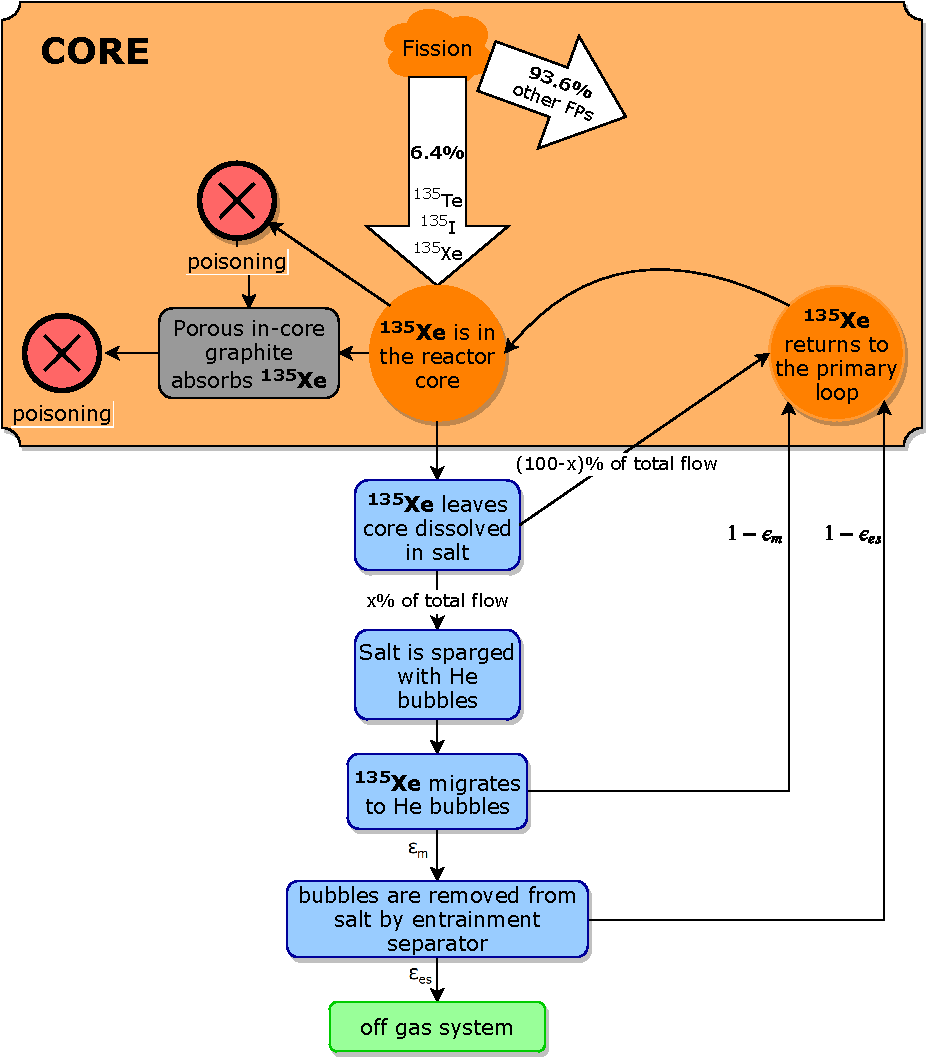
\includegraphics[width=\textwidth]{xe_diagram.pdf}
	\caption{Schematic $^{135}$Xe circulation diagram in a generic \gls{MSR}. 
	The $\epsilon_m$ is the migration efficiency of $^{135}$Xe to the helium 
	bubbles and $\epsilon_{es}$ is the gas separation efficiency in the 
	entrainment separator. The orange color represents the active core region, 
	the blue color represents the gas separation system, and the gray color is 
	moderator in the core. Fission yields listed for $^{235}$U.}
	\label{fig:xe_diagram}
\end{figure}
\begin{figure}[htp!] % replace 't' with 'b' to 
  \centering
  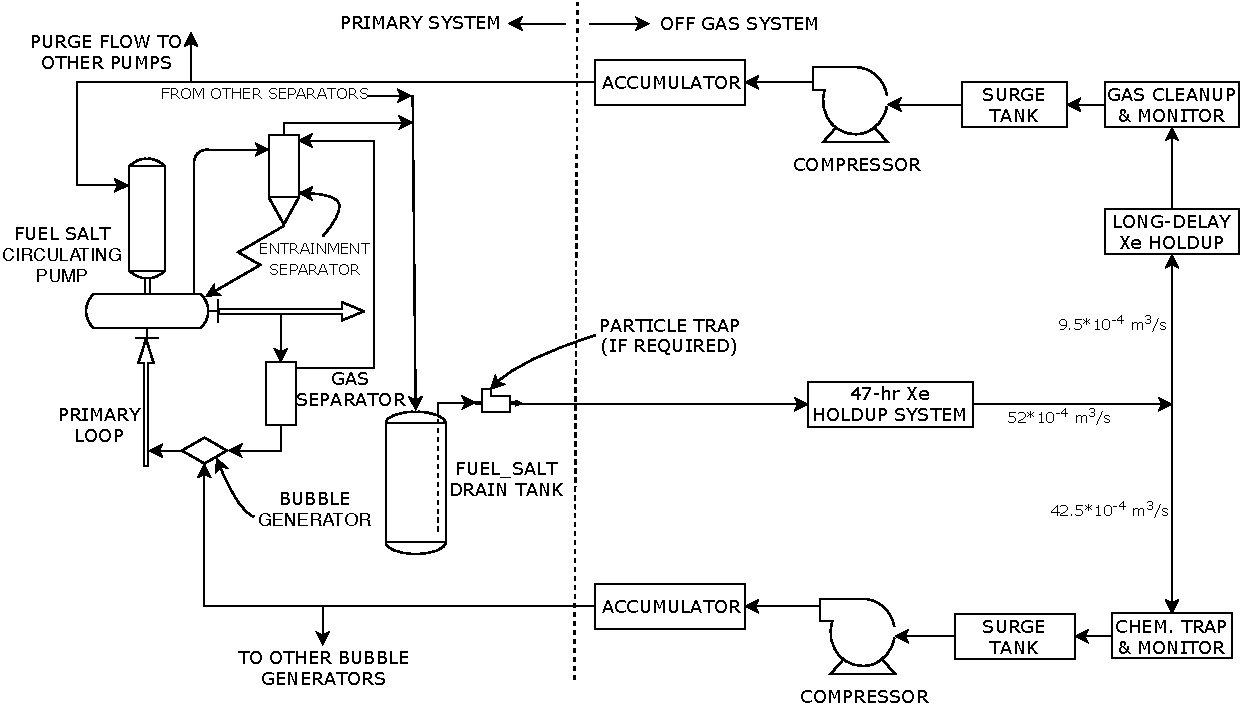
\includegraphics[width=\textwidth]{gas_separation.pdf}
  \caption{Schematic flow diagram of the \gls{MSBR} gas separation system 
  (figure reproduced from Robertson \emph{et al.} 
  \cite{robertson_conceptual_1971}).}
  \label{fig:gas_removal_system}
\end{figure}
\begin{figure}[htp!] % replace 't' with 'b' to 
  \centering
  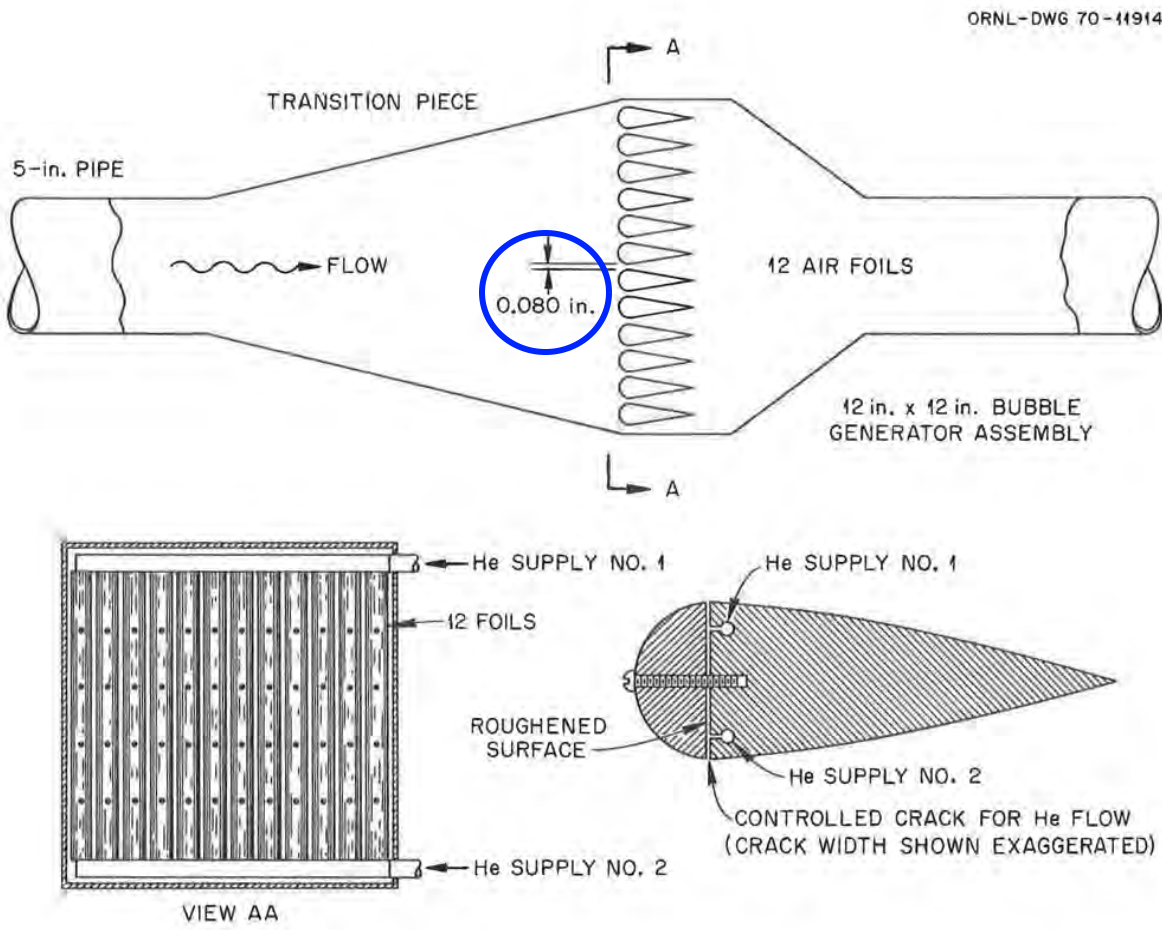
\includegraphics[width=0.77\textwidth]{msbr_bubble_generator.png}
  \caption{Preliminary concept of \gls{MSBR} bubble generator (figure 
  reproduced from Robertson \emph{et al.} \cite{robertson_conceptual_1971}). 
  The blue circle shows throat width, which determines bubble size.}
		\vspace{-0.25in}
  \label{fig:bubble_separator}
\end{figure}
\begin{table}[b]
	\caption{$^{135}$Xe loss terms and principal rate constants involved
		(reproduced from Kedl \emph{et al.} \cite{kedl_development_1967}).}
	\centering
	\begin{tabularx}{\textwidth}{b b}
		\hline \textbf{$^{135}$Xe loss mechanism}      & \textbf{Principal 
		rate 
			parameters involved}  	\\
		\hline Decay of dissolved $^{135}$Xe ($\tau_{1/2}=9.1$ h)  & Decay 
		constant	($\lambda$)		\\
		\hline $^{135}$Xe burnup              &  Neutron flux 
		($\Phi$)		 					\\
		dissolved xenon-135 burnup as it passes throught core  
		& 			            \\		\hline $^{135}$Xe transferred to 
		off-gas system via xenon stripper & Stripping efficiency 
		($\epsilon$)		\\
		\hline $^{135}$Xe transferred into circulating He bubbles; this xenon 
		will eventually be burnup, decay, or stripped via bubble separator & 
		Mass transfer coefficient ($h$), decay constant ($\lambda$), 
		neutron flux ($\phi$), bubble removing efficiency ($\epsilon$)		\\
		\hline 
	\end{tabularx}
	\label{tab:xe_loss}
\end{table}

To realistically model the gas separation system, a mathematical model 
describing noble gas extraction efficiency dynamics during reactor operation 
is required. Particularly, a model of xenon extraction efficiency as a 
function of a sparger design parameters is needed to accurately model 
$^{135}$Xe removal in a fuel salt depletion simulation. The gain and loss 
terms for $^{135}$Xe dissolved in the fuel salt are listed in 
Tables~\ref{tab:xe_gain} and \ref{tab:xe_loss}. The stripping efficiency for 
the xenon in the pump bowl has been measured during the \gls{MSRE} but the 
technical report ORNL-4069 by Kedl-Houtzeel only stated its range (from 50 to 
100\%) and mentioned that the results are not accurate 
\cite{kedl_development_1967}. $^{135}$Xe burnup and decay rates are well 
known. 

Peebles \emph{et al.} in ORNL-TM-2245 has reported xenon removal efficiency 
($\epsilon_{Xe}$) in a gas separation system as a function of many parameters 
\cite{peebles_removal_1968}:
\begin{align}
& \qquad\qquad \epsilon_{Xe} = \frac{1-e^{-\beta}}{1+\alpha}
	\intertext{where}
 	\alpha &= \frac{RTQ_{salt}}{HQ_{He}} \\
 	\beta &= \frac{K_L a A_C L (1+\alpha)}{Q_{salt}} \\
 	R &= \mbox{universal gas constant} \nonumber \\
 	T &= \mbox{salt temperature} \nonumber \\
 	Q_{salt}&= \mbox{volumetric salt flow rate} \nonumber \\
 	Q_{He}&= \mbox{volumetric helium flow rate} \nonumber \\
 	H &= \mbox{Henry's law constant for solute gas} \nonumber \\
 	a &= \mbox{gas-liquid interfacial area} \nonumber \\
 	A_C &= \mbox{contactor cross section} \nonumber \\
 	L &= \mbox{contactor length} \nonumber \\
  	K_L &= \mbox{liquid phase mass transfer coefficient} \nonumber
\end{align}
Most of input parameters for that correlation are obvious and easy to obtain 
from the system component design. The mass transfer coefficient for 
transferring xenon into helium bubbles ($K_L$) can be estimated from 
experiment or CFD-model but published information is insufficient to inform an 
accurate mathematical model\footnote{Peebles \emph{et al.} reported the mass 
transfer coefficient correlation for the \gls{MSBR} salt 
(LiF-BeF$_2$-ThF$_4$-UF$_4$) but for limited case. While it is out of the 
scope of this work to accurately estimate mass transfer coefficient, this work 
seeks to provide tool which will allow user to specify any mathematical model 
for a separation efficiency.}.

This technique would be applicable to other noble gases (e.g. Kr) but the 
mass transfer coefficients would be different. Current effort at the 
University of Illinois at Urbana-Champaign namely, ``Enabling Load Following 
Capability in the Transatomic Power \gls{MSR}" \cite{huff_enabling_2018}, have 
a goal to determine mass transfer coefficients for various gaseous \glspl{FP}  
using CFD simulations and verify them in small experiments. As a result, the 
obtained mathematical model for a gas removal efficiency will be used to 
inform realistic physics-based fuel reprocessing model in the proposed 
SaltProc tool.

\subsection{Fuel salt chemical processing facility} \label{sec:chemical_processing}
Additionally to noble gas (e.g., Xe, Kr), the fuel salt reprocessing system  
must extract other \glspl{FP}: noble/semi-noble metals and lanthanides. They  
generally have a relatively low capture cross section and thus absorb fewer 
neutrons than $^{135}$Xe, but their removal is crucial to guarantee normal  
operation. Some fraction of noble and semi-noble solid fission products are 
plate out onto a internal surfaces of the primary loop equipment. Lanthanides 
have relatively high solubility in the carrier salt and must be removed by 
chemical extraction. 

Protactinium presents another challenge for thorium-fueled 
\glspl{MSR}\footnote{$^{232}$Th in the fuel salt absorbs thermal neutrons 
and produces $^{233}$Pa which then decays into the fissile $^{233}$U 
($\tau_{1/2}=26.967d$).} (e.g., \gls{MSBR}, \gls{MSFR}), since it has a large 
absorption cross section in  the thermal energy spectrum. Accordingly, 
$^{233}$Pa is continuously removed from the fuel salt into a protactinium
decay tank to allow $^{233}$Pa to decay to $^{233}$U without poisoning the 
reactor. This feature allows the thorium-fueled \gls{MSR} to avoid neutron 
losses to protactinium, keeps fission products to a very low level, and 
increases the efficiency of $^{233}$U breeding. 

Many authors reported liquid-liquid reductive extraction process as a best 
option for removing protactinium and soluble fission products from 
molten fluoride salts \cite{briggs_molten-salt_1969, delpech_molten_2010, 
doligez_coupled_2014}. In that process the protactinium or lanthanides can be 
selectively stripped from the salt into liquid bismuth due to different 
chemical potentials. Moreover, the \gls{MSRE} studies indicated that the 
extraction could be carried out rapidly and continuously  
\cite{whatley_engineering_1970-1}.

The principal scheme of the \gls{MSBR} reprocessing facility concept is shown 
in Figure~\ref{fig:material_flow}. The fuel salt is first temporarily stored 
for cooling and decay of the shortest lived fission products, then directed to 
the primary fluorinator. There most of the uranium is removed by fluorination 
to UF$_6$. After that, the salt is routed to an extraction column where the 
mixture containing metallic bismuth, lithium and thorium as reductants is 
contacted with the salt. The remaining uranium and protactinium are 
reductively extracted to a bismuth solution, leaving a salt that only contains 
fission products dissolved in carrier salt (base composition 
LiF-BeF$_2$-ThF$_4$). The salt then goes through a reduction column where 
UF$_6$ is reduced to UF$_4$ in the salt and preparing it for return to the 
reactor. BeF$_2$ and ThF$_4$ are also added and all residual bismuth is 
removed from the salt. After a final cleanup step and valence adjustment, the 
purified salt returns to the reactor \cite{carter_design_1972, 
sorensen_one-fluid_2006}.
\begin{figure}[htp!] % replace 't' with 'b' to 
  \centering
  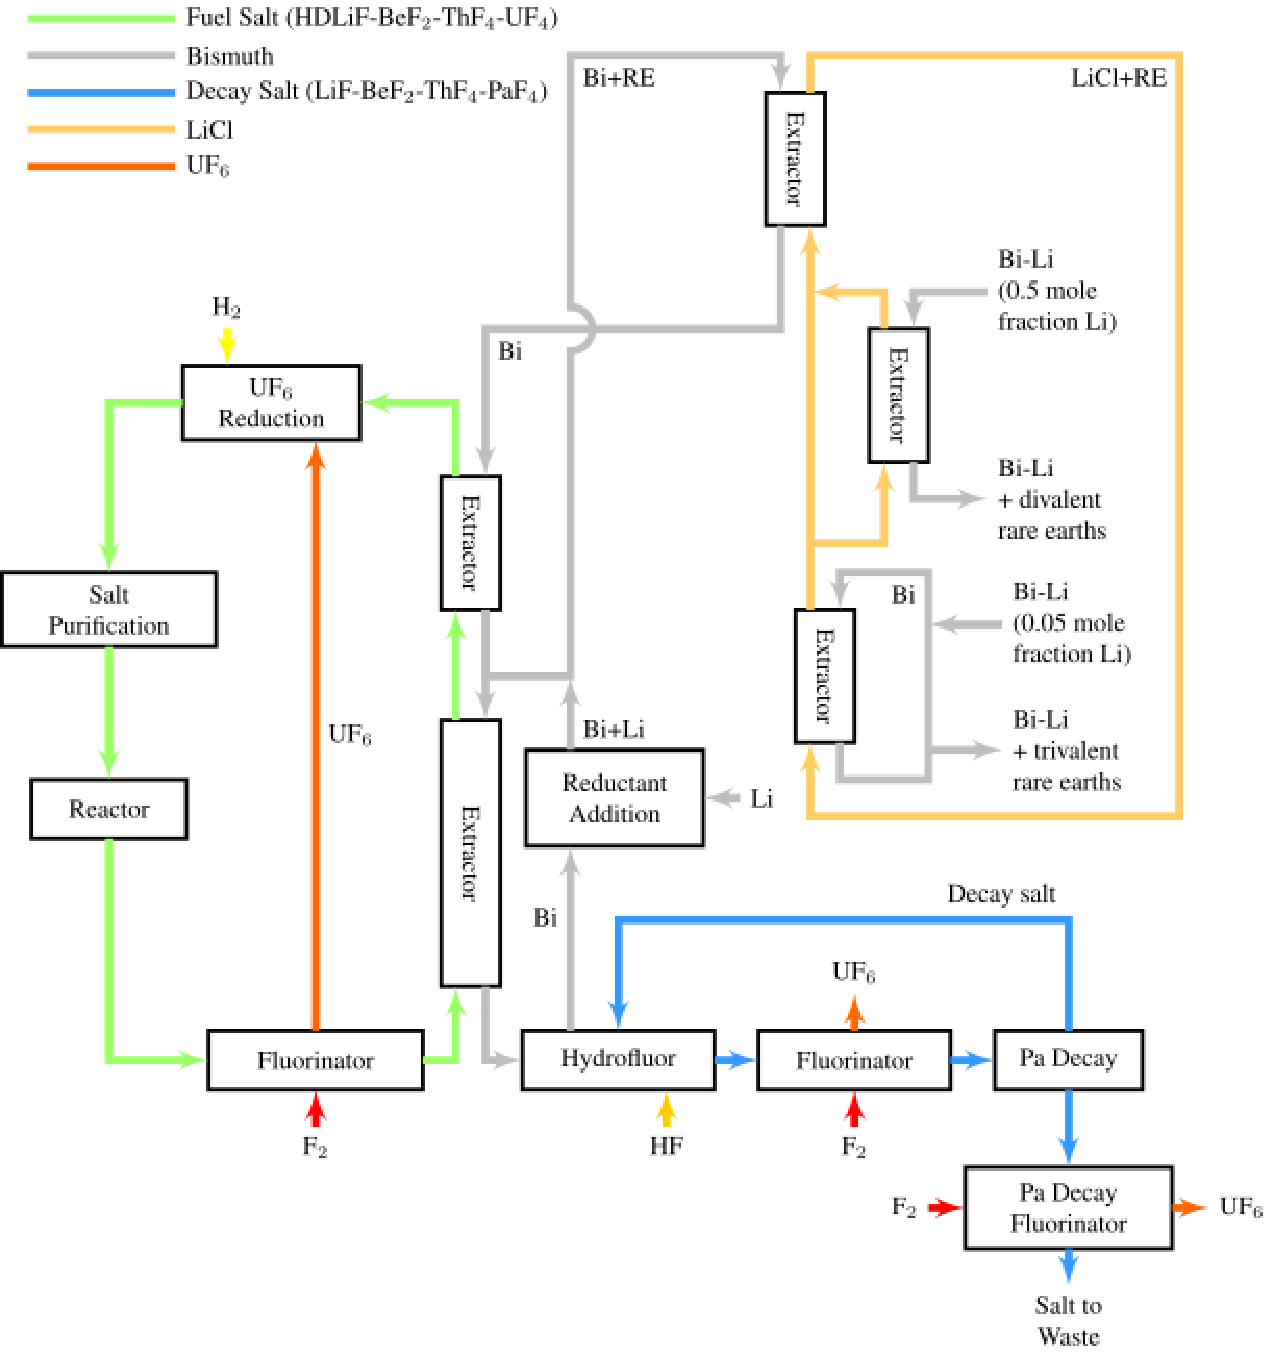
\includegraphics[width=1.05\textwidth]{flowsheet.pdf}
  \caption{Simplified block diagram of chemical processing scheme for 
  single-fluid \gls{MSBR} (reproduced from Sorensen 
  \cite{sorensen_one-fluid_2006}). \emph{RE} is a reducing agent.}
  \label{fig:material_flow}
\end{figure}

The bismuth accommodating some uranium and protactinium is routed to a 
hydrofluorination column where metallic solutes in the bismuth are 
oxidized into their fluoride forms in the presence of a decay 
salt\footnote{The decay salt contains UF$_4$, PaF$_4$, ThF$_4$ and fission 
products. Uranium produced after $^{233}$Pa decay is extracted and directed 
back into the reactor. Decay salt is the precursor for the waste salt as it 
was periodically discarded every 220 days.}. The decay salt, containing 
UF$_4$, PaF$_4$, and ThF$_4$, passed into a decay tank where $^{233}$Pa is 
decays to $^{233}$U. The uranium generated by protactinium decay is removed 
through fluorination to UF$_6$ and directed to the reduction column to refuel 
the purified fuel salt. A hydrofluorinator and a fluorinator can remove 
approximately 95\% of the uranium from the stream 
\cite{robertson_conceptual_1971}.

The fully processed salt, on its way back to the reactor, has uranium added 
from the protactinium decay tank at the rate required to maintain or adjust 
the uranium concentration in the reactor (and, consequently, control the 
reactivity). Adding fissile material is performed by sparging the salt with 
UF$_6$ and hydrogen to produce UF$_4$ in the salt and HF gas 
\cite{robertson_conceptual_1971}.

The fuel salt stream from the protactinium isolation system contains only 
traces of protactinium and uranium (because it was separated in the system) 
but contains practically all of the rare earths. A fraction of this salt 
stream is redirected to a reductive extraction process for removing rare 
earths.  The principal scheme of a rare earth removal system is shown in 
Figure~\ref{fig:rare-earth-removal}. A molten salt flow which contains 
rare-earth fluorides is fed to the center of an extraction column. The salt 
flows countercurrent to a liquid bismuth stream which contains thorium and 
lithium. In the upper part of the column, the rare earths are reduced and 
transferred to the downflowing liquid metal stream. Below the feed point, the 
rare earth concentration is increased in the salt and metal streams in order 
to produce a concentration high enough for disposal 
\cite{briggs_molten-salt_1969}.
\begin{figure}[htbp!]
	\centering
	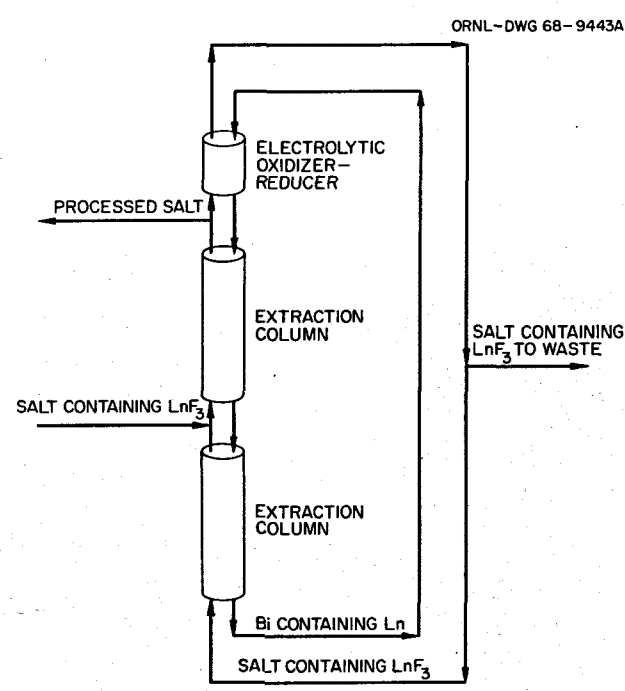
\includegraphics[width=0.45\textwidth]{rare-earths-removal-system.png}
	\caption{Rare earth removal from a fuel salt by reductive extraction 
	(figure reproduced from Briggs \emph{et al.} 
	\cite{briggs_molten-salt_1969}).}
	\label{fig:rare-earth-removal}
\end{figure}

Molten salt leaving the top of the column contains a dilute concentration of 
rare earths. A fraction of this flow is returned back to the reactor while the 
rest is sent to an electrolytic cell complex. The net effect of the complex is 
to push thorium and lithium into bismuth and to return extracted rare earths, 
entering the complex with bismuth from the bottom of the cascade, to the 
cascade as reflux, oxidizing them out of the metal and transferring them to 
the returning salt stream.

While it is out of the scope of proposed work to derive accurate 
chemistry-based mathematical formula for \glspl{FP} separation efficiency, 
this work seeks to provide a flexible tool that would be able to simulate 
chemical processes in a high-detailed level.

\section{Serpent overview}
Serpent is a continuous-energy Monte Carlo neutronics software capable of 
solving the neutron transport problem by tracking individual neutrons within 
the problem geometry and using stochastic method to determine chain of events 
for each neutron \cite{leppanen_serpent_2015}. Serpent has been under active 
development at the VTT Technical Research Centre of Finland since 2004, where 
it was initially conceived as a tool to simplify group constant generation in 
a high-fidelity Monte Carlo environment. Serpent is now widely used transport 
code  with a growing user base. Now Serpent used by more than 500 registered 
individuals in 155 organizations located in 37 countries around the world. The 
burnup calculation capability in Serpent is based on built-in calculation 
routines, without using any external solvers. A restart feature allows 
performing fuel shuffling or applying any modifications in the input by 
dividing the calculation into several parts, which is crucial for online 
reprocessing simulations.

The latest version, Serpent 2, supports advanced geometries and has advanced 
burnup capabilities, including online refueling capabilities which are 
necessary for neutronic computations of pebble-bed reactors and liquid-fueled 
\glspl{MSR} \cite{aufiero_extended_2013}. Unfortunately, built-in online 
refueling features are still under active development and unavailable to 
ordinary users. Furthermore, recently multi-physics simulations using Serpent  
2 were demonstrated, including  calculations with thermal-hydraulics, 
\gls{CFD} and fuel performance codes \cite{leppanen_numerical_2015}. Two-way 
coupling to thermal-hydraulics, \gls{CFD}, and fuel performance codes operates 
on two levels: internal coupling to built-in solvers for fuel behavior and 
thermal-hydraulics and external coupling via a universal multi-physics 
interface. 

Serpent 2 can be effectively run in parallel on computer clusters and 
multi-core workstations. Parallelization is handled by thread-based OpenMP, 
which enables all processsors to use shared memory space. Calculations can be 
divided into several nodes by distributed-memory \gls{MPI} parallelization. 
Serpent 2  is an improvement upon Serpent 1, and contains a complete redesign 
of memory management using hybrid OpenMP \cite{dagum_openmp_1998} + \gls{MPI} 
parallelization.  This hybrid parallelization is important in depletion 
calculations using computer clusters with multiple nodes, and allows to 
achieve significant speed-up in depletion calculations on computer clusters 
with more than 4'000 cores \cite{leppanen_serpent_2015}. 

All calculations herein were performed using Serpent 2 version 2.1.31 on Blue 
Waters’ XE6 nodes. For cross section generation, the JEFF-3.1.2 nuclear data 
library was employed based on entirely open cross section data 
\cite{oecd/nea_data_bank_jeff-3.1.2_2014}. 

\section{Proposed simulation tool design and capabilities} \label{sec:tool_design}
The first version of the SaltProc Python tool for calculating \gls{MSR} fuel 
composition evolution taking into account an online reprocessing system 
was developed in 2018 as a part of M.S. thesis \cite{rykhlevskii_advanced_2018,
	rykhlevskii_arfc/saltproc_2018}. The tool was designed to 
expand Serpent 2 depletion capabilities for modeling liquid-fueled \gls{MSR} 
with online fuel reprocessing system. SaltProc v1 uses HDF5 
\cite{the_hdf_group_hierarchical_1997} to store 
data and uses the PyNE Nuclear Engineering Toolkit \cite{scopatz_pyne_2012}
for Serpent 2 output file parsing and nuclide naming. SaltProc v1 is an 
open-source Python package that uses a batch-wise approach to simulate 
continuous feeds and removals in \glspl{MSR}. 

SaltProc v1 only allows 100\% separation efficiency for either specific 
elements or groups of elements at the end of the specific ``cycle 
time''\footnote{The \gls{MSBR} program defined ``cycle time'' as the time 
required to remove 100\% of a target nuclide from a fuel salt 
\cite{robertson_conceptual_1971}.}. Capabilities of the developed tool, 
working with the Monte Carlo software Serpent 2, were demonstrated using the 
full-core MSBR design for a simplified case with ideal removal efficiency 
(100\% of mass for target elements removed) \cite{rykhlevskii_modeling_2019}. 
The SaltProc v1 architecture and principal structure was not designed for 
flexible implementation of sophisticated online reprocessing systems including 
realistic variable extraction efficiencies. 

For the proposed work, SaltProc v1 will be completely re-factored using 
\gls{OOP} to create a comprehensive generic tool to realistically model 
complex \gls{MSR} fuel reprocessing system while taking into account 
variable extraction efficiencies, time-dependent core geometry, mass balance 
between the core and the reprocessing plant.

\subsection{Proposed software architecture}
The SaltProc v2.0+ Python toolkit will couple directly with Serpent 2 input 
and output files, to allow the reprocessing system couples to depletion 
calculation. Existing PyNE interfaces will be employed for Serpent output 
parsing as well as newly developed interfaces for input and output handling. 
Python 3 \gls{OOP} standard features will be used to create a flexible, 
user-friendly tool with great potential for further improvement and 
collaboration. Figure~\ref{fig:saltproc_class} shows the proposed SaltProc 
v2.0+ class structure which includes 4 main classes:
\begin{figure}[ht!] % replace 't' with 'b' to \centering
	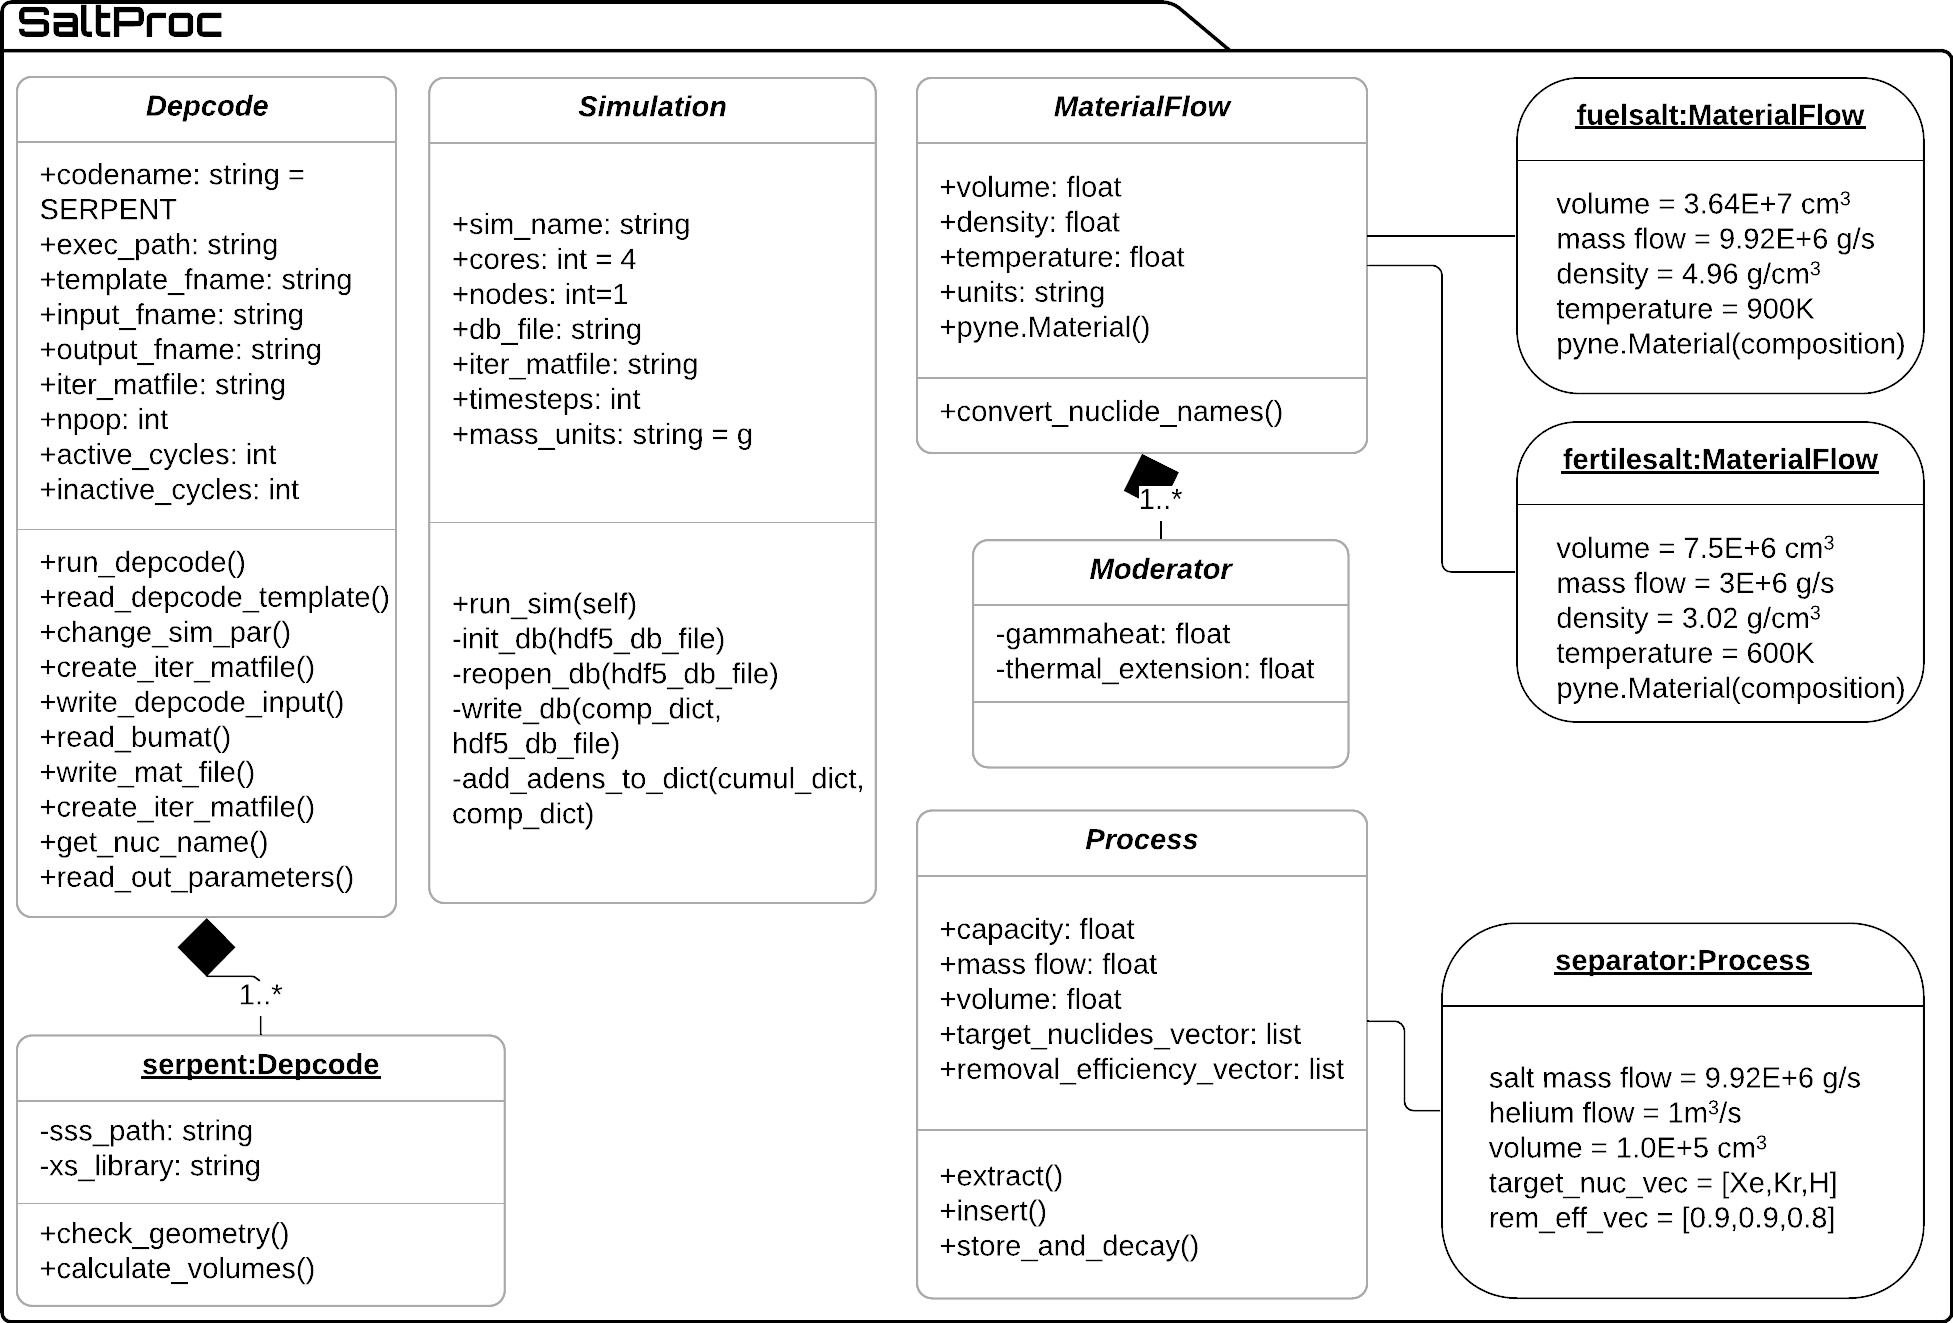
\includegraphics[width=1.03\textwidth]{saltproc_class_diagram.png}
	\vspace{-0.15in}
	\caption{SaltProc v2.0+ python package class diagram in UML notation 
		and examples of object instances.}
	\label{fig:saltproc_class}
\end{figure}
\paragraph{Depcode.}Contains attributes and methods for reading the user's 
input file for the depletion software, initial material (e.g., fuel and/or 
fertile salt) composition, principal parameters for burnup simulation (e.g., 
neutron population and number of cycles for Monte Carlo neutron transport), 
and running the depletion code.
\paragraph{Simulation.}Runs Serpent depletion step, creates and writes HDF5 
database, tracks time and converts isotopic composition vector nuclide names 
from Serpent to human-readable format.
\paragraph{MaterialFlow.}Each \textit{MaterialFlow} object 
represents the material flowing between \textit{Process} objects. 
All instances of this class contain an isotopic composition vector 
(PyNE Material object initialized from Serpent output file \textbf{dep.m}), 
mass flow rate, temperature, density, volume, and void fraction. Existing PyNE 
Material capabilities allows to easily convert the units of isotopic  
composition vector (e.g., from atomic density provided by Serpent to 
a mass fraction or absolute mass in desired units), decay material 
(i.e. model the \gls{MSBR} protactinium decay tank), calculate 
decay heat, activity, and dose. The main idea of the \textit{MaterialFlow} 
object is to pass detailed information about the salt starting at the 
\gls{MSR} vessel outlet throughout reprocessing components 
(\textit{Processes}), which modify the \textit{MaterialFlow} 
object before depleting the material in the next Serpent burnup step.
\paragraph{Process.}Each \textit{Process} object represents a 
realistic fuel processing step characterized by its throughput rate, 
volumetric capacity, extraction efficiency for each target element (can be 
a function of many parameters), waste streams, and other parameters specific 
to the particular process. Feed	\textit{Process} injects fresh fuel salt 
\textit{MaterialFlow} directly into the reactor core (e.g., adding fissile 
material with a specific mass flow rate to \textit{MaterialFlow} after 
performing all removals).

The proposed class structure provides outstanding flexibility in simulating 
various \gls{MSR} fuel processing system designs. A library of various  
\textit{MaterialFlow} (e.g., fuel salt flow, fertile salt flow, refueling salt 
flow) and \textit{Process} (e.g., helium sparging facility, gas separator, 
lanthanide removal component) objects will be created to allow a user to 
quickly create a model of a desired reprocessing scheme. At runtime, the user 
will connect \textit{Process} objects in series or parallel with 
\textit{MaterialFlow} objects to form a comprehensive reprocessing system. The 
user will also be able to create custom objects with desired attributes and 
methods, and contribute back to the code package using GitHub 
(https://github.com/arfc/saltproc).	

\subsection{Tentative flowchart}
Figure~\ref{fig:saltproc_flow} illustrates the proposed online reprocessing 
simulation algorithm coupling SaltProc v2.0+ and Serpent. To perform a 
depletion step, SaltProc v2.0+ reads a user-defined Serpent template file. 
This file contains input parameters such as geometry, material, isotopic 
composition, neutron population, criticality cycles, total heating power, and 
boundary conditions. SaltProc v2.0+ fills in the template file and runs 
Serpent single-step depletion. After the depletion calculation, SaltProc v2.0+ 
reads the depleted fuel composition file into \textit{MaterialFlow} object  
(\textit{core\textunderscore outlet} in figure~\ref{fig:saltproc_flow}). This 
object contains an isotopic composition vector, total volume of material, 
total mass, mass flow rate, density, temperature, void fraction, etc. For the 
simplest reprocessing case, when all fuel processing components are located 
in-line (100\% of total material flow goes through a chain of separation 
components), the \textit{core\textunderscore outlet} 
object is flowing sequentially between \textit{Processes} and each 
\textit{Process} is removing a mass fraction of target elements with specified 
extraction efficiency. Afterward, the removed material mass is compensated by 
fresh fuel salt to maintain the salt inventory in a primary loop. 
Finally, resulting isotopic composition after reprocessing is stored in 
HDF5 database and dumped in a new composition file for the next 
Serpent depletion run. SaltProc v2.0+ also stores in database isotopic  
composition before reprocessing and waste stream from each fuel processing 
component. 
\begin{figure}[ht!] % replace 't' with 'b' to \centering
	\centering
	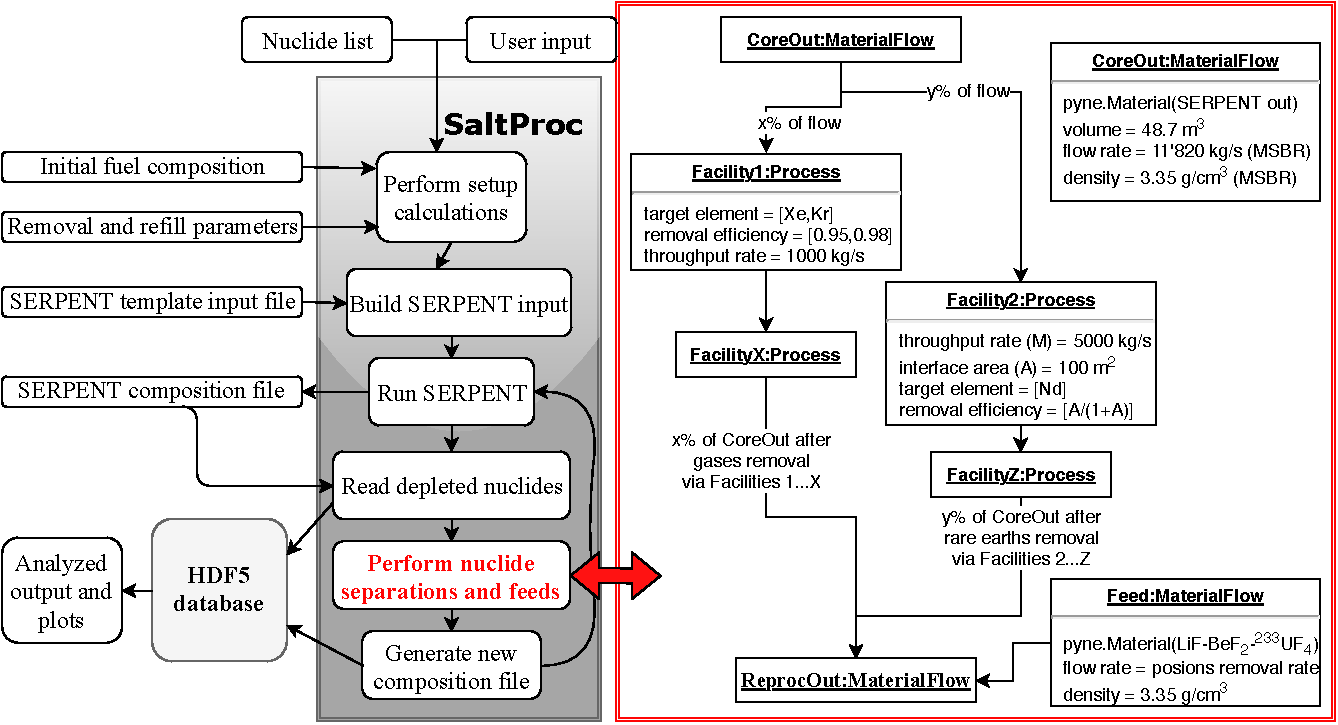
\includegraphics[width=1.05\textwidth]{saltproc_flowchart.pdf}
	\vspace{-0.15in}
	\caption{Tentative generic flow chart for SaltProc v2.0+ python package.}
	\label{fig:saltproc_flow}
\end{figure}

For a more general case with multiple concurrent extraction processes, a 
separate \textit{MaterialFlow} object is created for each branch with a 
user-defined mass flow rate (e.g. 90\% of total mass flow rate flows via left 
branch and 10\% throughout a right branch). The total mass and isotopic 
composition vector for each \textit{MaterialFlow} object is calculated as a 
fraction of incoming \textit{core\textunderscore outlet} flow. Then each 
\textit{MaterialFlow} object is passed via a cascade of \textit{Processes} to 
separate selected chemical elements with specific efficiency. Finally, the 
left-hand-side branch \textit{MaterialFlow} object is merged with the 
right-hand-side and similarly to the previous case, fresh fuel salt feed 
compensate the loss of mass in separation facilities and keep fuel salt mass 
in a primary loop constant.

The class diagram (Figure~\ref{fig:saltproc_class}) allows to model the 
operation of a complex, multi-zone, multi-fluid \gls{MSR} and is sufficiently 
general to represent myriad reactor systems. The re-factored version of 
SaltProc will only store and edit the isotopic composition of the fuel stream, 
which makes it a flexible tool to model any geometry: an infinite medium, a 
unit cell, a multi-zone simplified assembly, or a full core. This flexibility 
allows the user to perform simulations of varying fidelity and computational 
intensity. SaltProc v2.0+ is an open-source tool (but a user needs Serpent 
2.1.31 installed to use SaltProc v2.0+), available on Github. It leverage unit 
and continuous tests  crucial for sustainable development  
\cite{krekel_pytest_2004}. It will also have documentation generated through 
Sphinx, a documentation generator, for ease of use \cite{brandl_sphinx_2009}. 
In summary, the development approach of SaltProc v2.0+ is focused on producing 
a generic, flexible and expandable tool to give the Serpent 2 Monte Carlo code 
the ability to conduct advanced in-reactor fuel cycle analysis as well as 
simulate many online refueling and fuel reprocessing systems.

%\subsection{Reactivity control module}
%In addition, SaltProc will be able to define time-dependent material feed and 
%removal rates to investigate their impacts. These rates need not be 
%constant in SaltProc. They can be defined as piecewise functions or set to 
%respond to conditions in the core. For instance, SaltProc might increase the 
%fissile material feeding rate if the effective multiplication factor, 
%$k_{eff}$, falls below a specific limit (e.g., 1.002).
%These capabilities allow SaltProc to analyze fuel cycle of a generic 
%liquid-fueled \gls{MSR}.

\section{Preliminary results}
Developed as a part of my master thesis, the first version of the tool only 
was able to leverage ideal removals (e.g., 100\% of target isotope mass 
extracted). The capabilities of SaltProc was demonstrated for full-core 
\gls{MSBR} model \cite{rykhlevskii_modeling_2019}. 
Subsection~\ref{sec:msbr_reproc} summarized a preliminary work and results 
obtained from applying a previous version of SaltProc to the \gls{MSBR} core 
and reprocessing plant.

\subsection{MSBR online reprocessing analysis} \label{sec:msbr_reproc}
The \gls{MSBR} vessel has a diameter of 680 cm and a height of 610 cm. It 
contains a molten fluoride fuel-salt mixture that generates heat in the active 
core region and transports that heat to the primary heat exchanger by way of 
the primary salt pump. In the active core region, the fuel salt flows through 
channels in moderating and reflecting graphite blocks.  
Figure~\ref{fig:serpent_plan_view} shows the configuration of the 
\gls{MSBR} vessel, including the ``fission" (zone I) and ``breeding" 
(zone II) regions inside the vessel. The core has two radial zones bounded by 
a solid cylindrical graphite reflector and the vessel wall. The central zone, 
zone I, in which 13\% of the volume is fuel salt and 87\% graphite, is
composed of 1,320 graphite cells, 2 graphite control rods, and 2 
safety\footnote{ These rods needed for emergency shutdown only.} rods. The 
under-moderated zone, zone II, with 37\% of fuel salt, and the radial 
reflector, surrounds the zone I core region and serves to diminish neutron 
leakage. Zones I and II are surrounded radially and axially by fuel salt 
(figure~\ref{fig:serpent_zoneII}). This space for fuel is necessary for 
injection and flow of molten salt.
\begin{figure}[ht!] % replace 't' with 'b' to 
	\centering
	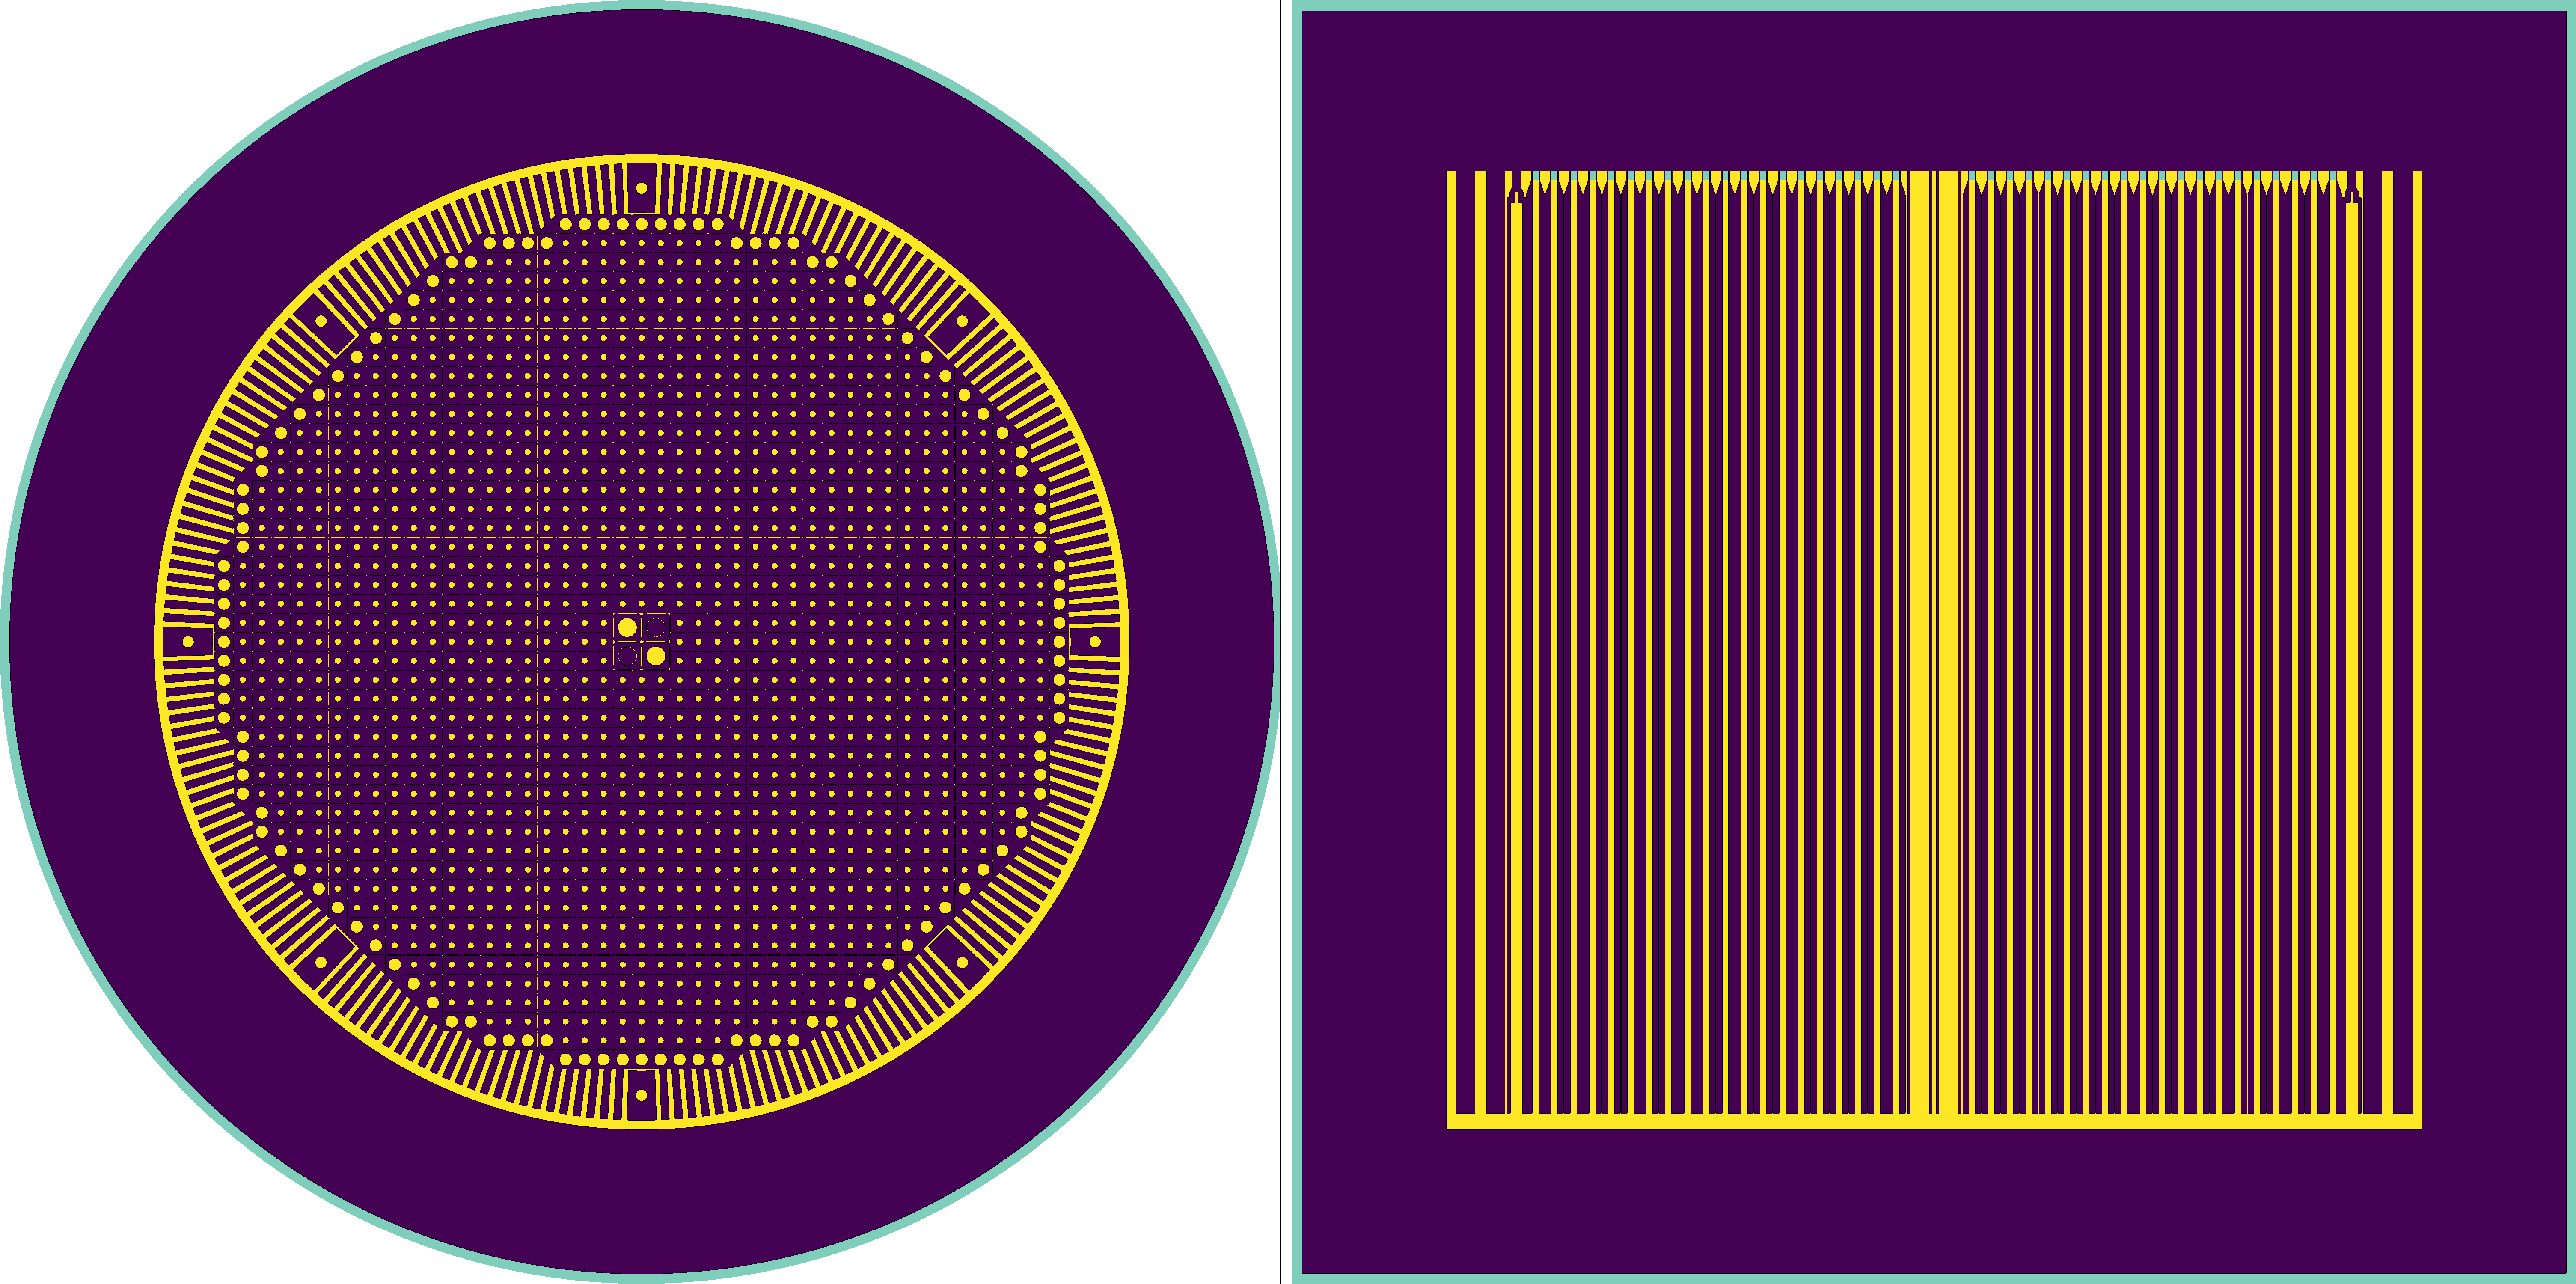
\includegraphics[width=\textwidth]{view_serpent.png}
	\caption{$XY$ (left) and $XZ$ (right) views of Serpent \gls{MSBR} model 
		(figure reproduced from \cite{rykhlevskii_full-core_2017}).}
	\label{fig:serpent_plan_view}
\end{figure}
\begin{figure}[hb!] % replace 't' with 'b' to 
	\centering
	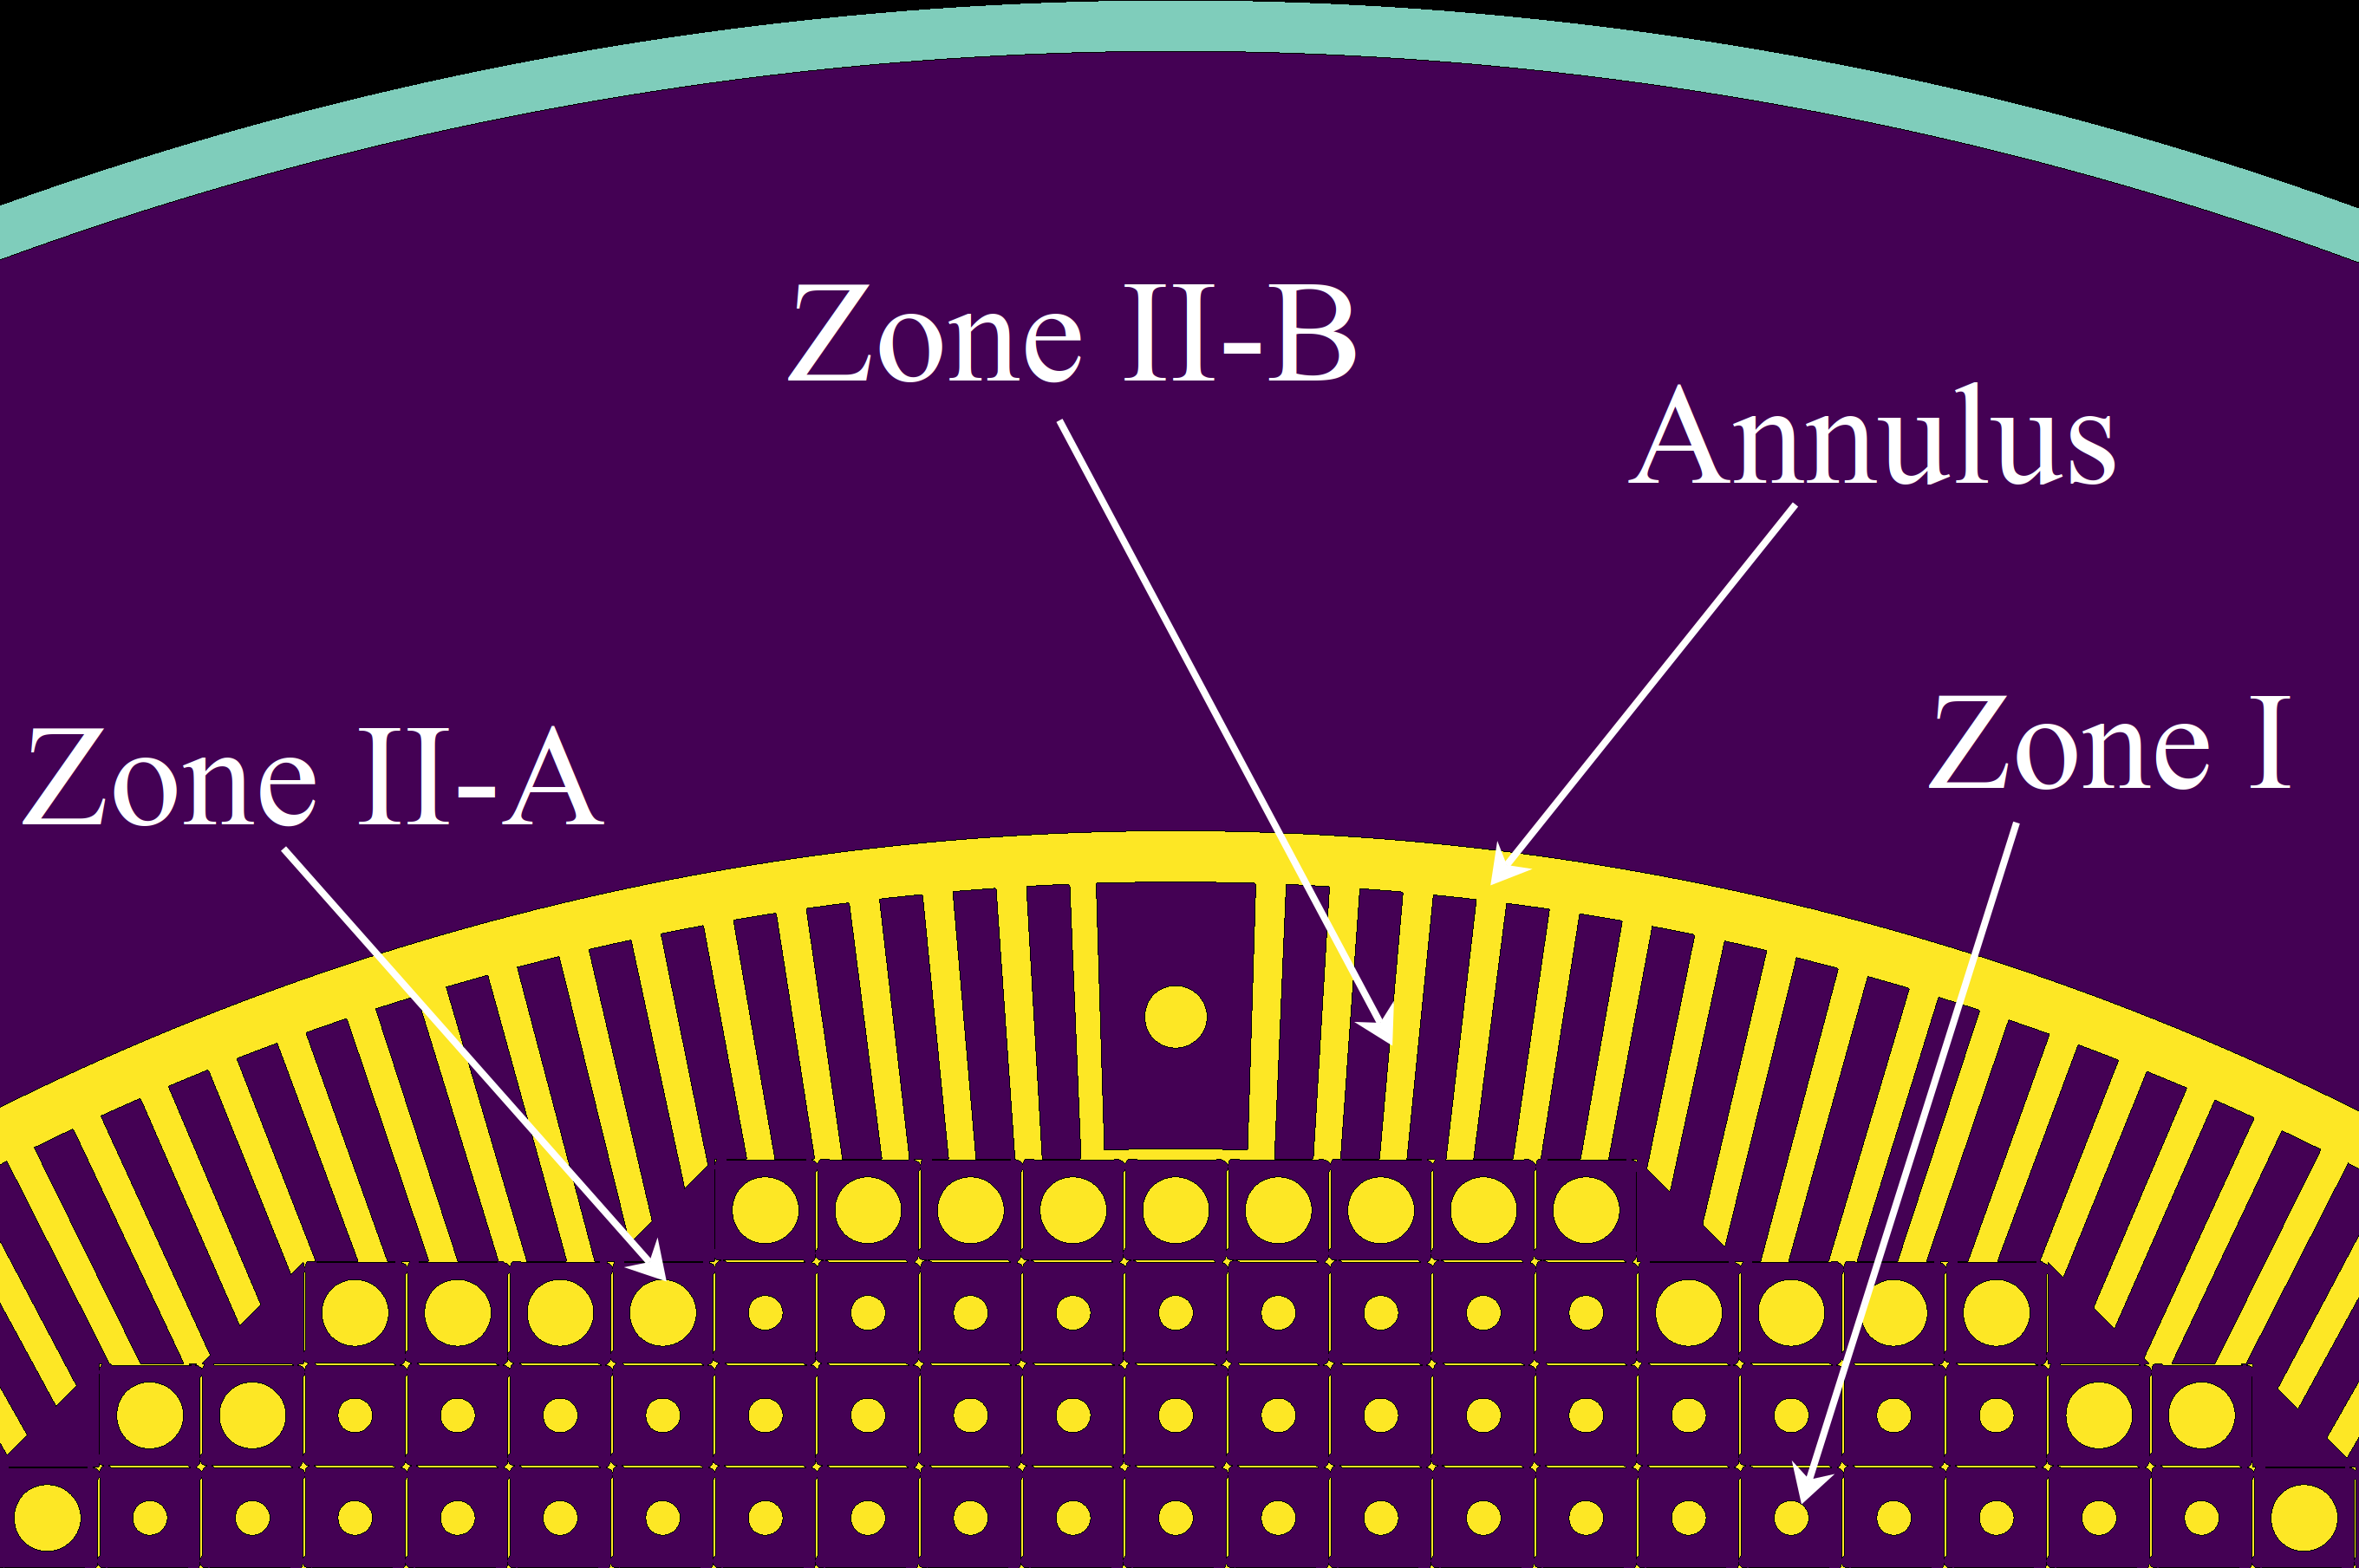
\includegraphics[width=0.7\textwidth]{ser_zone_II.png}
	\caption{Detailed view of \gls{MSBR} two zone model. 
		Yellow represents fuel salt, purple represents graphite, and aqua 
		represents the reactor vessel. Figure reproduced from 
		\cite{rykhlevskii_full-core_2017}.}
	\label{fig:serpent_zoneII}
\end{figure}

The \gls{MSBR} design requires online reprocessing to remove neutron gaseous 
\glspl{FP} (Xe, Kr) and noble metals (e.g., Se, Nb, Mo) every 20 seconds. 
$^{233}$Pa is continuously removed from the fuel salt into a protactinium 
decay tank to allow $^{233}$Pa to decay to $^{233}$U without the corresponding 
negative neutronics impact. This feature allows the reactor to avoid neutron 
losses to protactinium, lowers in-core fission product inventory, and 
increases the efficiency of $^{233}$U breeding. 
Table~\ref{tab:reprocessing_list_msbr} summarizes a full list of 
nuclides and the cycle time used for modeling salt treatment and separations 
\cite{robertson_conceptual_1971}. The removal rates vary among nuclides in 
this reactor concept and dictate the necessary resolution of depletion 
calculations. If the depletion time intervals are very short, an enormous 
number of depletion steps are required to obtain the equilibrium composition. 
On the other hand, if the depletion  calculation time interval is too long, 
the impact of short-lived fission products is not captured. To compromise, a 3 
day time interval was selected for depletion calculations to correlate with 
the removal interval of $^{233}$Pa, and $^{232}$Th was continuously added to 
maintain the initial mass fraction of $^{232}$Th.
%%%%%%%%%%%%%%%%%%%%%%%%%%%%%%%%%%%%%%%%
\begin{table}[ht!]
	\caption{The cycle times for protactinium and fission 
		products removal (reproduced from Robertson \emph{et al.} 
		\cite{robertson_conceptual_1971}).}
	\begin{tabularx}{\textwidth}{x  s  x}
		\hline Processing group & \qquad\qquad\qquad Nuclides & Cycle time (at 
		full power) \\ \hline Rare earths & Y, La, Ce, Pr, Nd, Pm, Sm, 
		Gd & 50 days \\ \qquad & Eu & 500 days \\ Noble metals & Se, 
		Nb, Mo, Tc, Ru, Rh, Pd, Ag, Sb, Te & 20 sec \\
		Seminoble metals & Zr, Cd, In, Sn & 200 days \\
		Gases & Kr, Xe & 20 sec \\ Volatile fluorides & Br, I & 60 days \\
		Discard & Rb, Sr, Cs, Ba & 3435 days \\ 
		%Salt discard & Th, Li, Be, F & 3435 days \\ 
		Protactinium & $^{233}$Pa & 3 days \\ Higher 
		nuclides & $^{237}$Np, $^{242}$Pu & 16 years \\  \hline
	\end{tabularx}
	\label{tab:reprocessing_list_msbr}
\end{table}
%%%%%%%%%%%%%%%%%%%%%%%%%%%%%%%%%%%%%%%%%

Figures~\ref{fig:keff} and \ref{fig:keff_zoomed} show the effective 
multiplication factors obtained using SaltProc and Serpent. The effective 
multiplication factors were calculated after removing fission products listed 
in Table~\ref{tab:reprocessing_list_msbr} and adding the fertile material at 
the end of cycle time (3 days for this work). The effective multiplication 
factor fluctuates significantly as a result of the batch-wise nature of this 
online reprocessing strategy. 
\begin{figure}[ht!] 
	\centering
	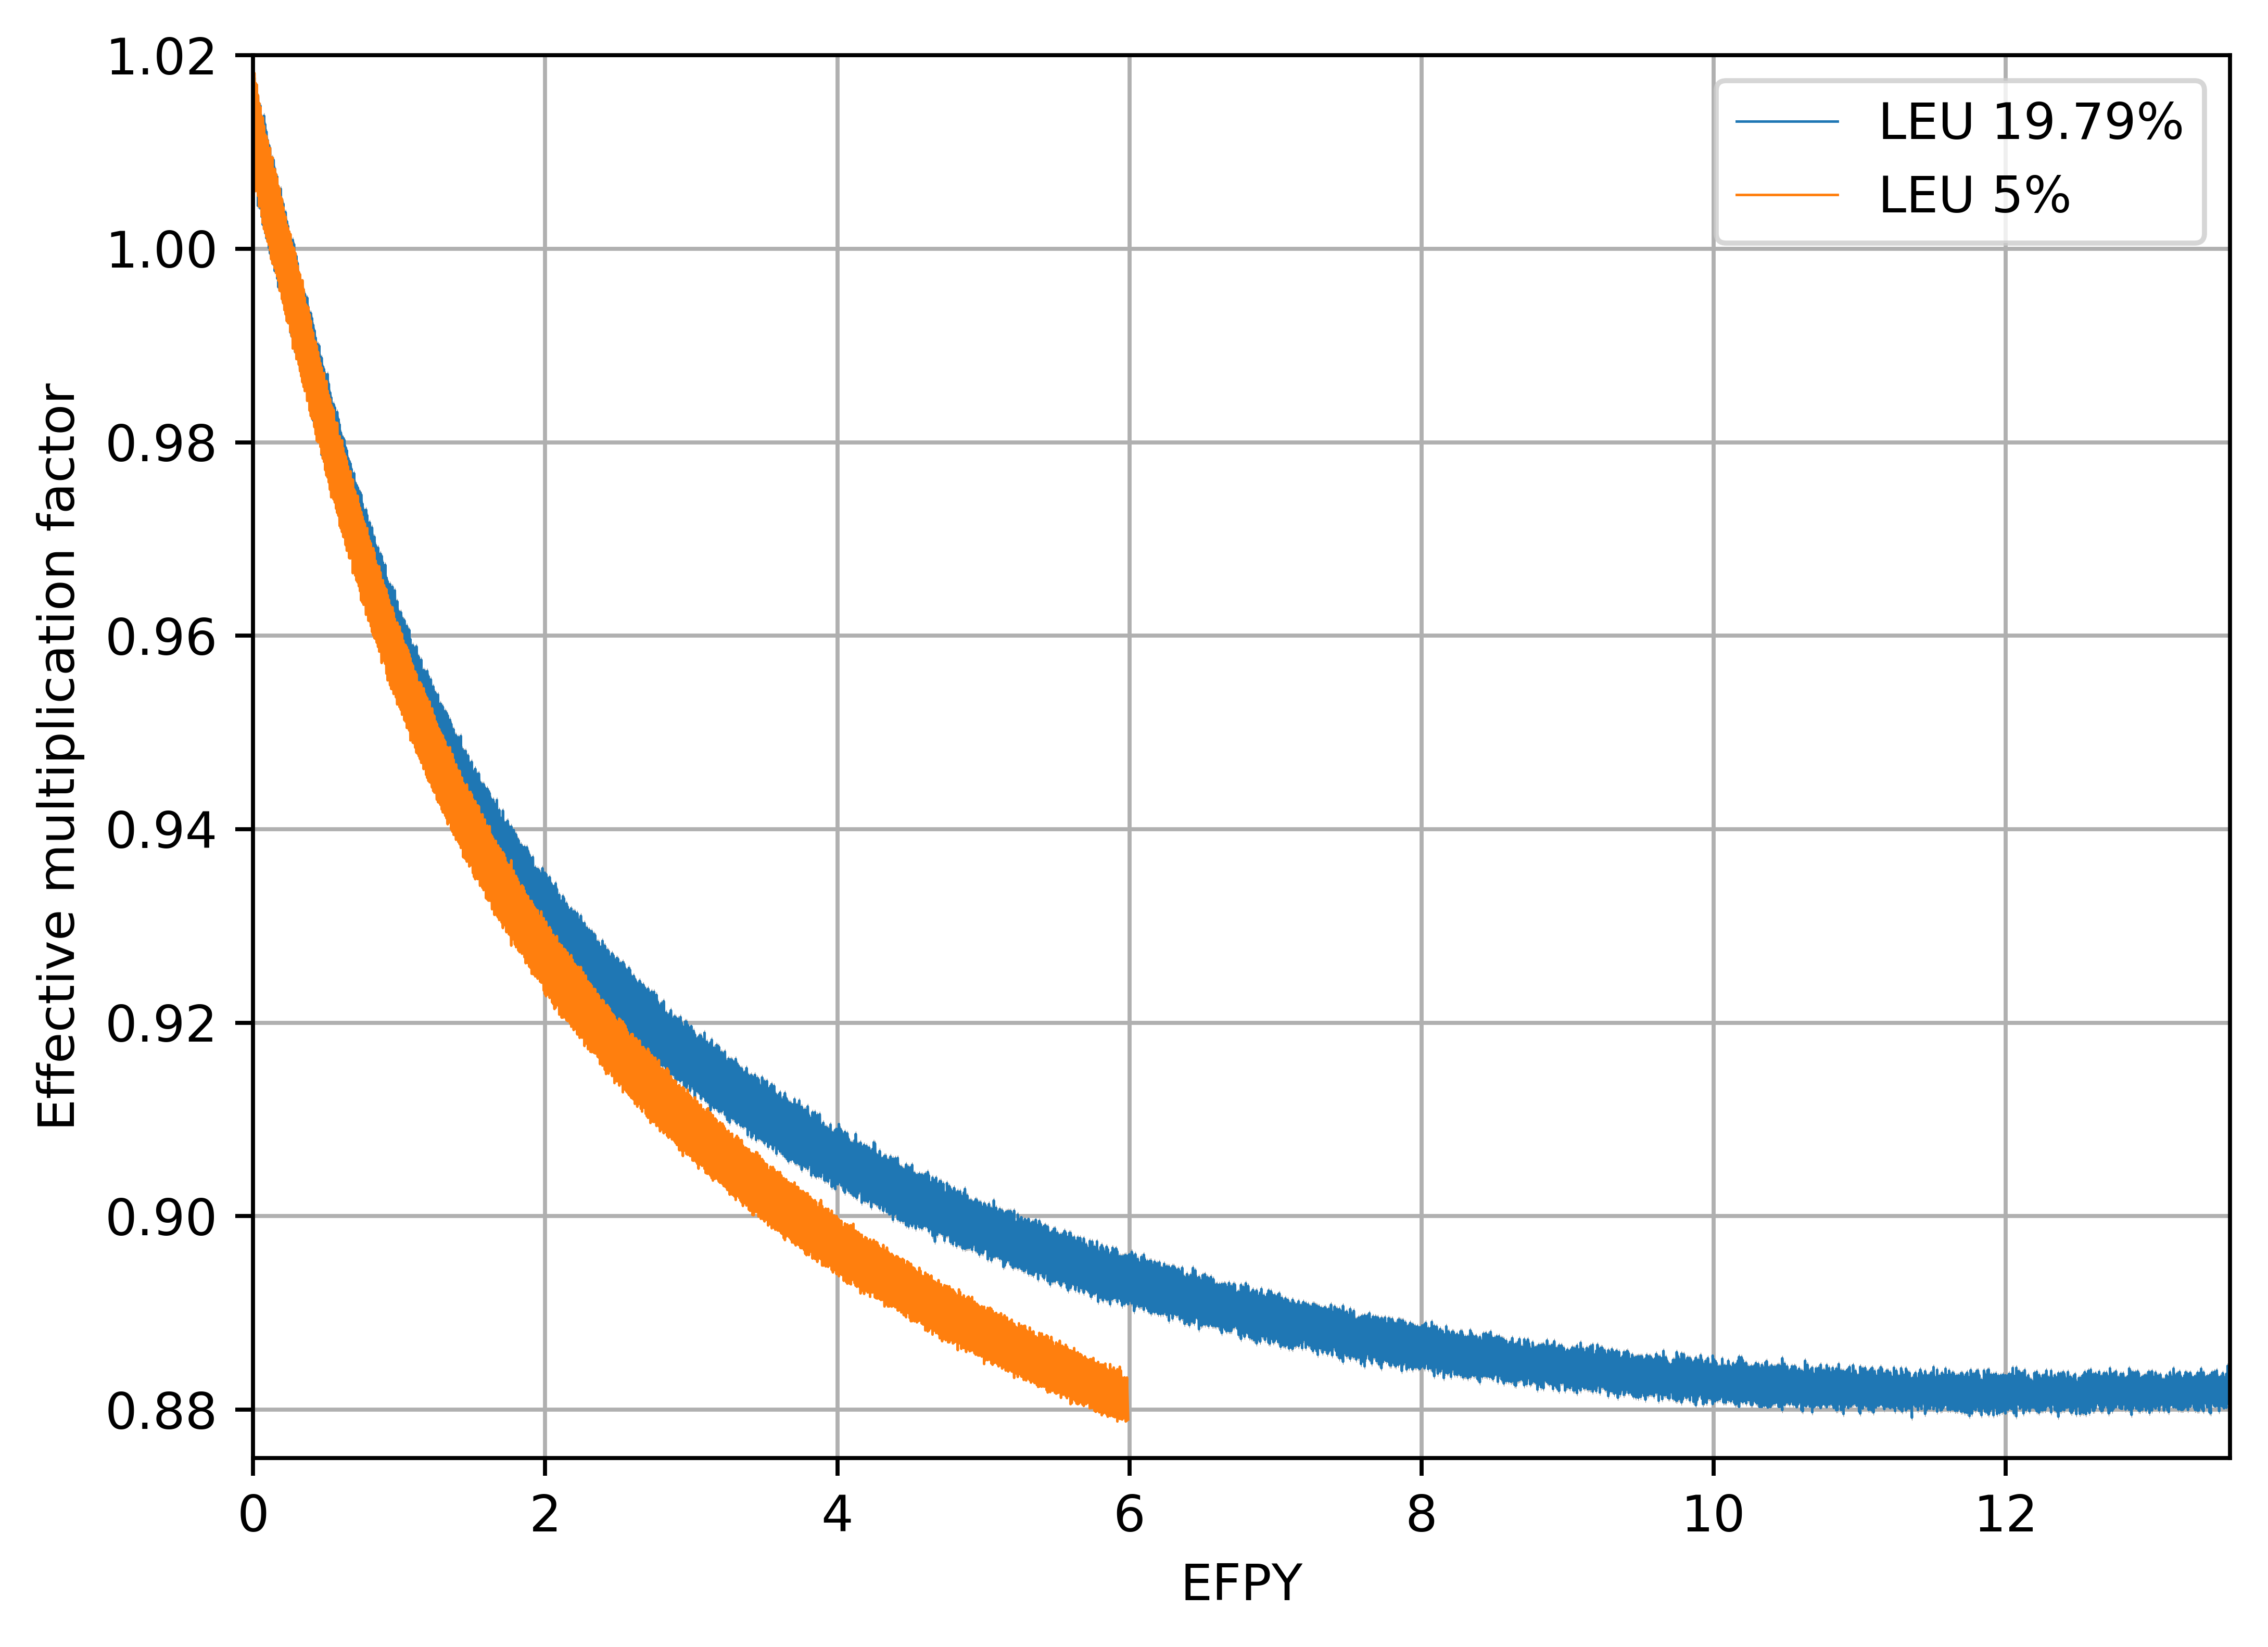
\includegraphics[width=0.9\textwidth]{keff.png}
	\caption{Effective multiplication factor dynamics for full-core \gls{MSBR} 
		model over a 60-year reactor operation lifetime (reproduced from 
		\cite{rykhlevskii_modeling_2019}).}
	\label{fig:keff}
\end{figure}
\begin{figure}[ht!] 
	\centering
	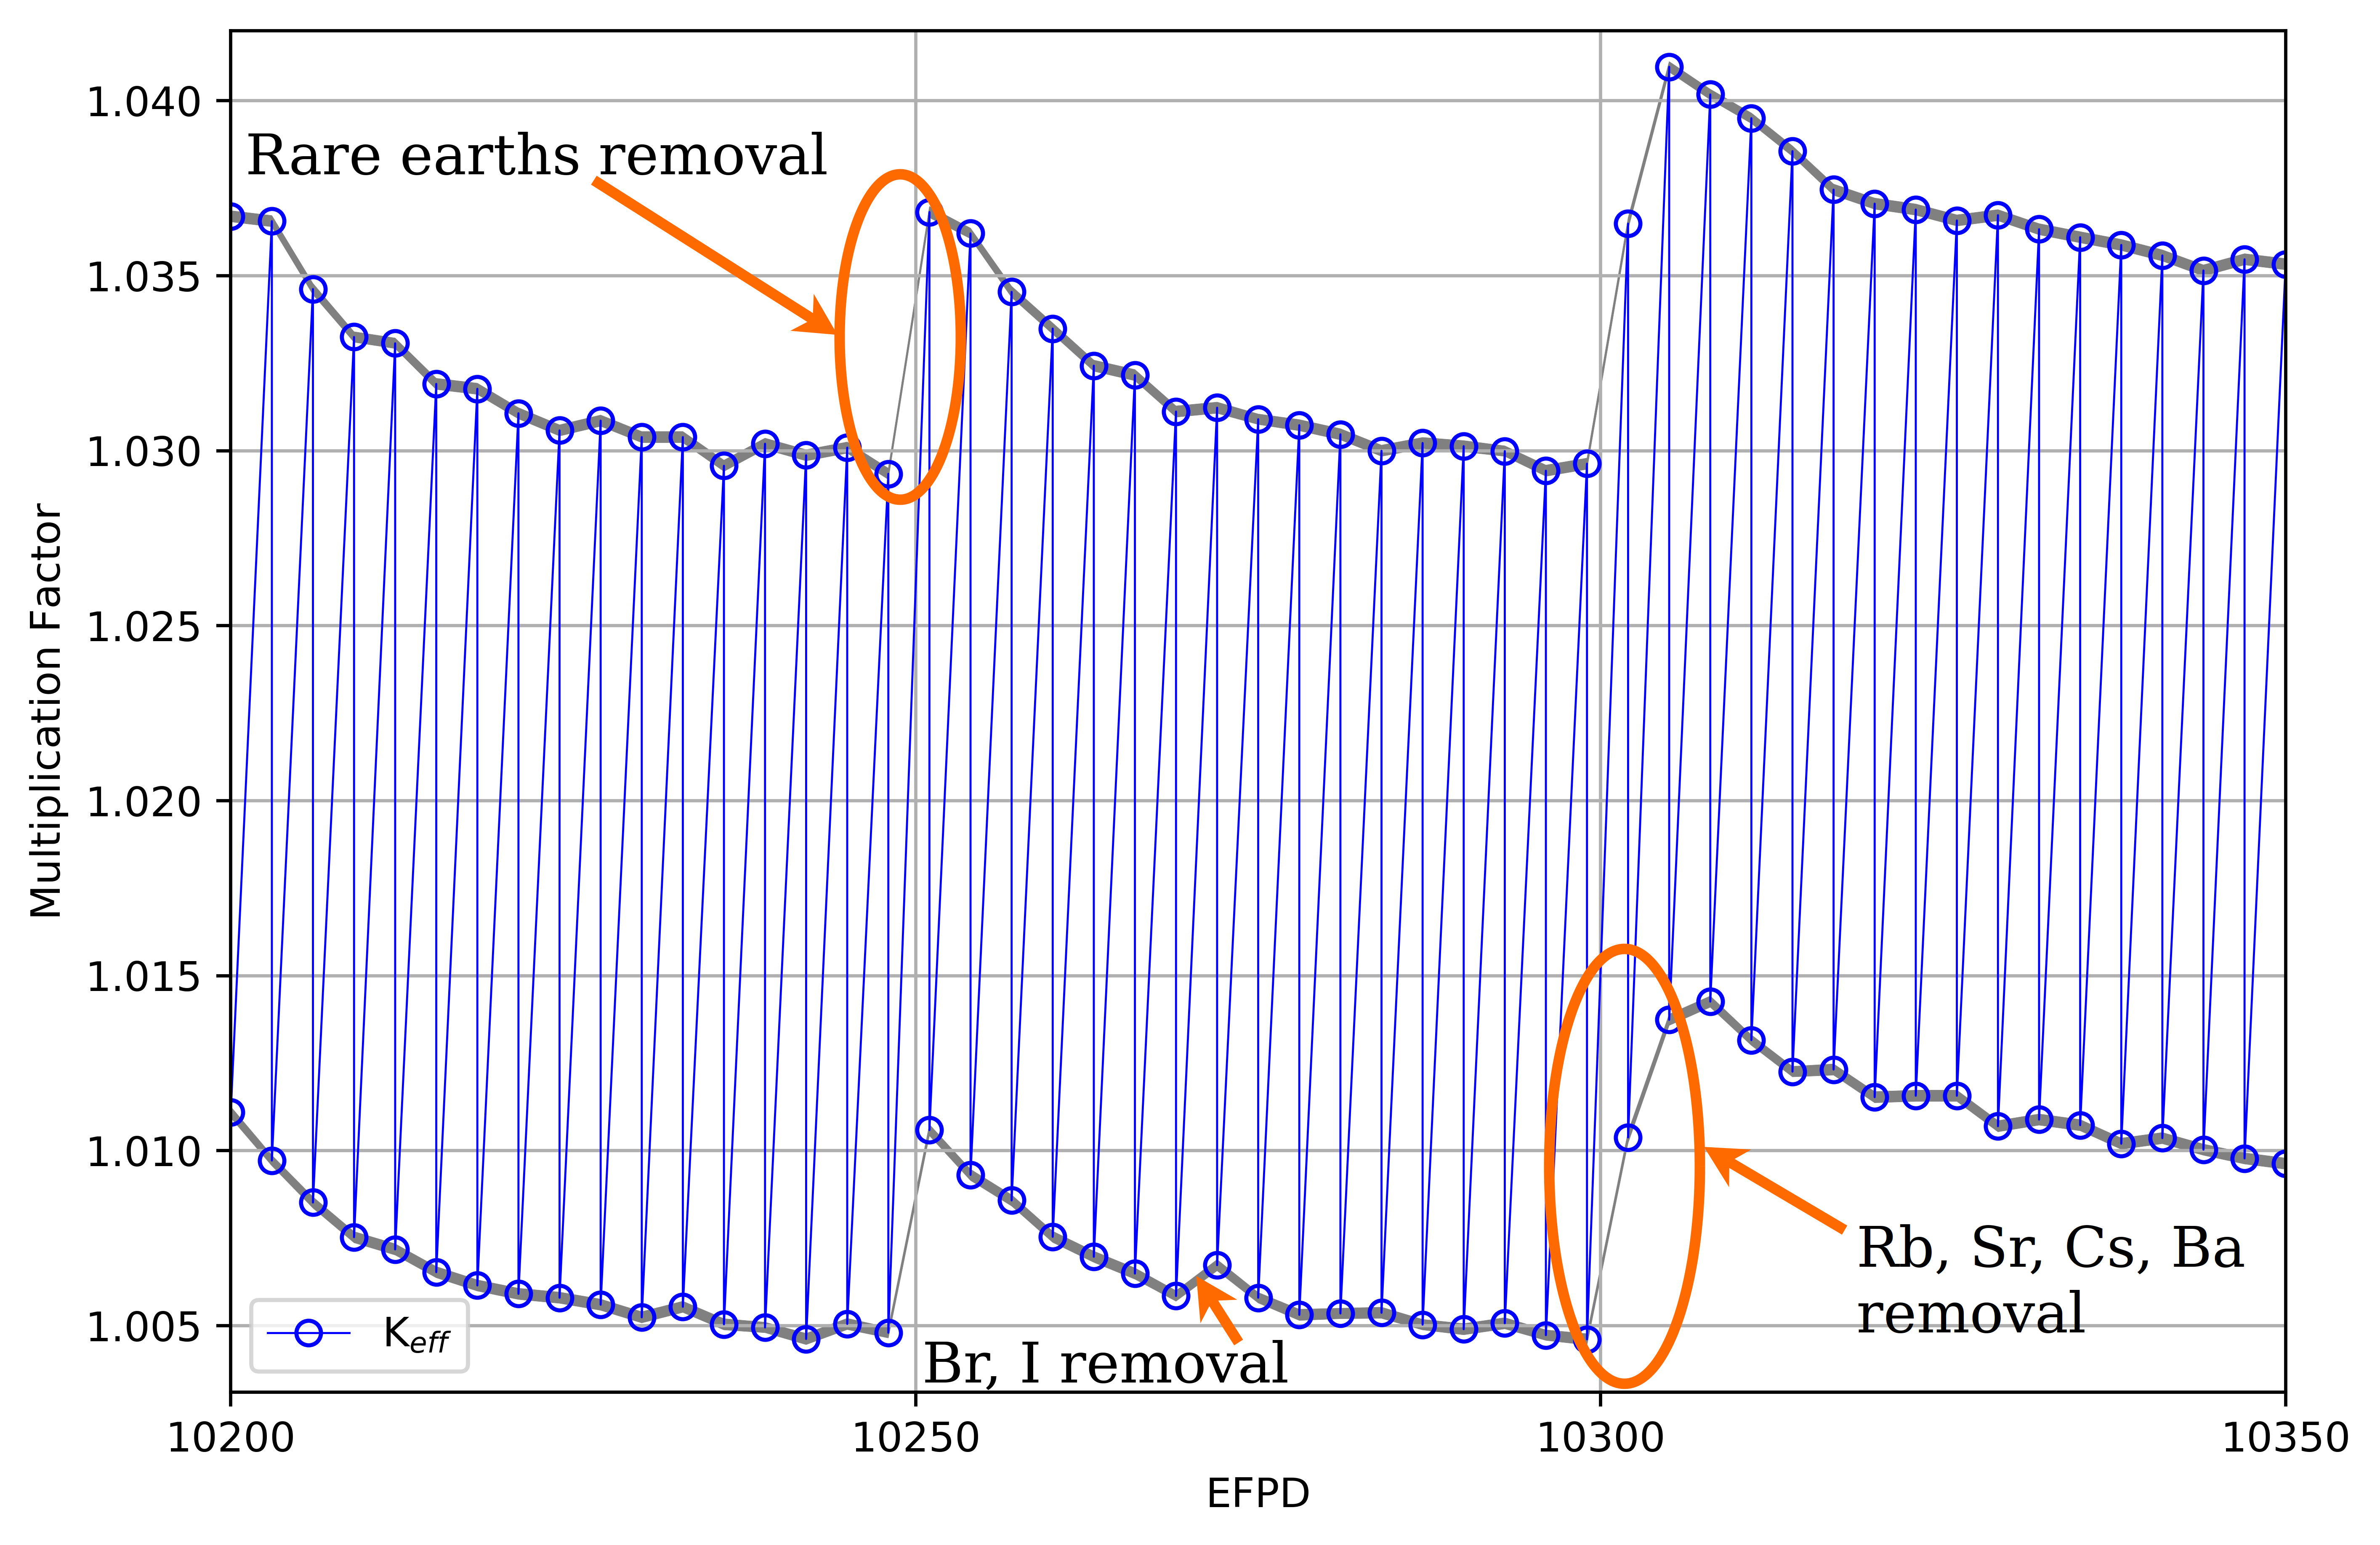
\includegraphics[width=\textwidth]{keff_zoomed.png}
	\caption{Zoomed effective multiplication factor for 150-EFPD time interval 
		(reproduced from \cite{rykhlevskii_modeling_2019}).}
	\label{fig:keff_zoomed}
\end{figure}

First, Serpent calculates the effective multiplication factor for the 
beginning of the cycle (there is fresh fuel composition at the first step). 
Next, it computes the new fuel salt composition at the end of a 3-day 
depletion. The corresponding effective multiplication factor is much smaller 
than the previous one. Finally, Serpent calculates $k_{eff}$ for the depleted 
composition after applying feeds and removals. The $k_{eff}$ increases 
accordingly since major reactor poisons (e.g. Xe, Kr) are removed, while fresh 
fissile material ($^{233}$U) from the protactinium decay tank is added.  

Additionally, the presence of rubidium, strontium, cesium, and barium in the 
core are disadvantageous to reactor physics. 
Overall, the effective multiplication factor gradually decreases from 1.075 to 
$\approx$1.02 at equilibrium after approximately 6 years of irradiation. 

Loading initial fuel salt composition into the \gls{MSBR} core leads to a 
supercritical configuration (Figure ~\ref{fig:fp_removal}). After reactor 
startup, the effective multiplication factor for the case with volatile gas 
and noble metal removal is approximately 7500 pcm  higher than for the case 
with no fission product removal. This significant impact on the reactor core is
achieved due to immediate removal (20 sec cycle time) of elements with a high 
absorption cross section (e.g., Xe, Kr, Mo). The effect of rare earth 
element removal was considerable a few months after startup and reached 
approximately 5500 pcm after 10 years of operation. The rare earth elements 
were removed at a slower rate (50-day cycle time). Moreover, 
Figure~\ref{fig:fp_removal} demonstrates that batch-wise removal of strong 
absorbers every 3 days did not necessarily lead to fluctuation in results 
but rare earth element removal every 50 days caused an approximately 600 pcm 
jump in reactivity.

The effective multiplication factor of the core reduces gradually over 
operation time because the fissile material ($^{233}$U) continuously depletes 
from the fuel salt due to fission while fission products simultaneously
accumulate in the fuel salt. Eventually, without fission product removal, 
the reactivity decreases to the subcritical state after approximately 500 and 
1300 days of operation for cases with no removal and volatile gas \& noble 
metal removal, respectively. The time when the simulated core reaches 
subcriticality ($k_{eff}<$1.0) for full-core model) is called the core 
lifetime. 
Therefore, removing fission products provides significant neutronic benefit 
and enables a longer core lifetime.
\begin{figure}[t] % replace 't' with 'b' to force it to 
	\centering
	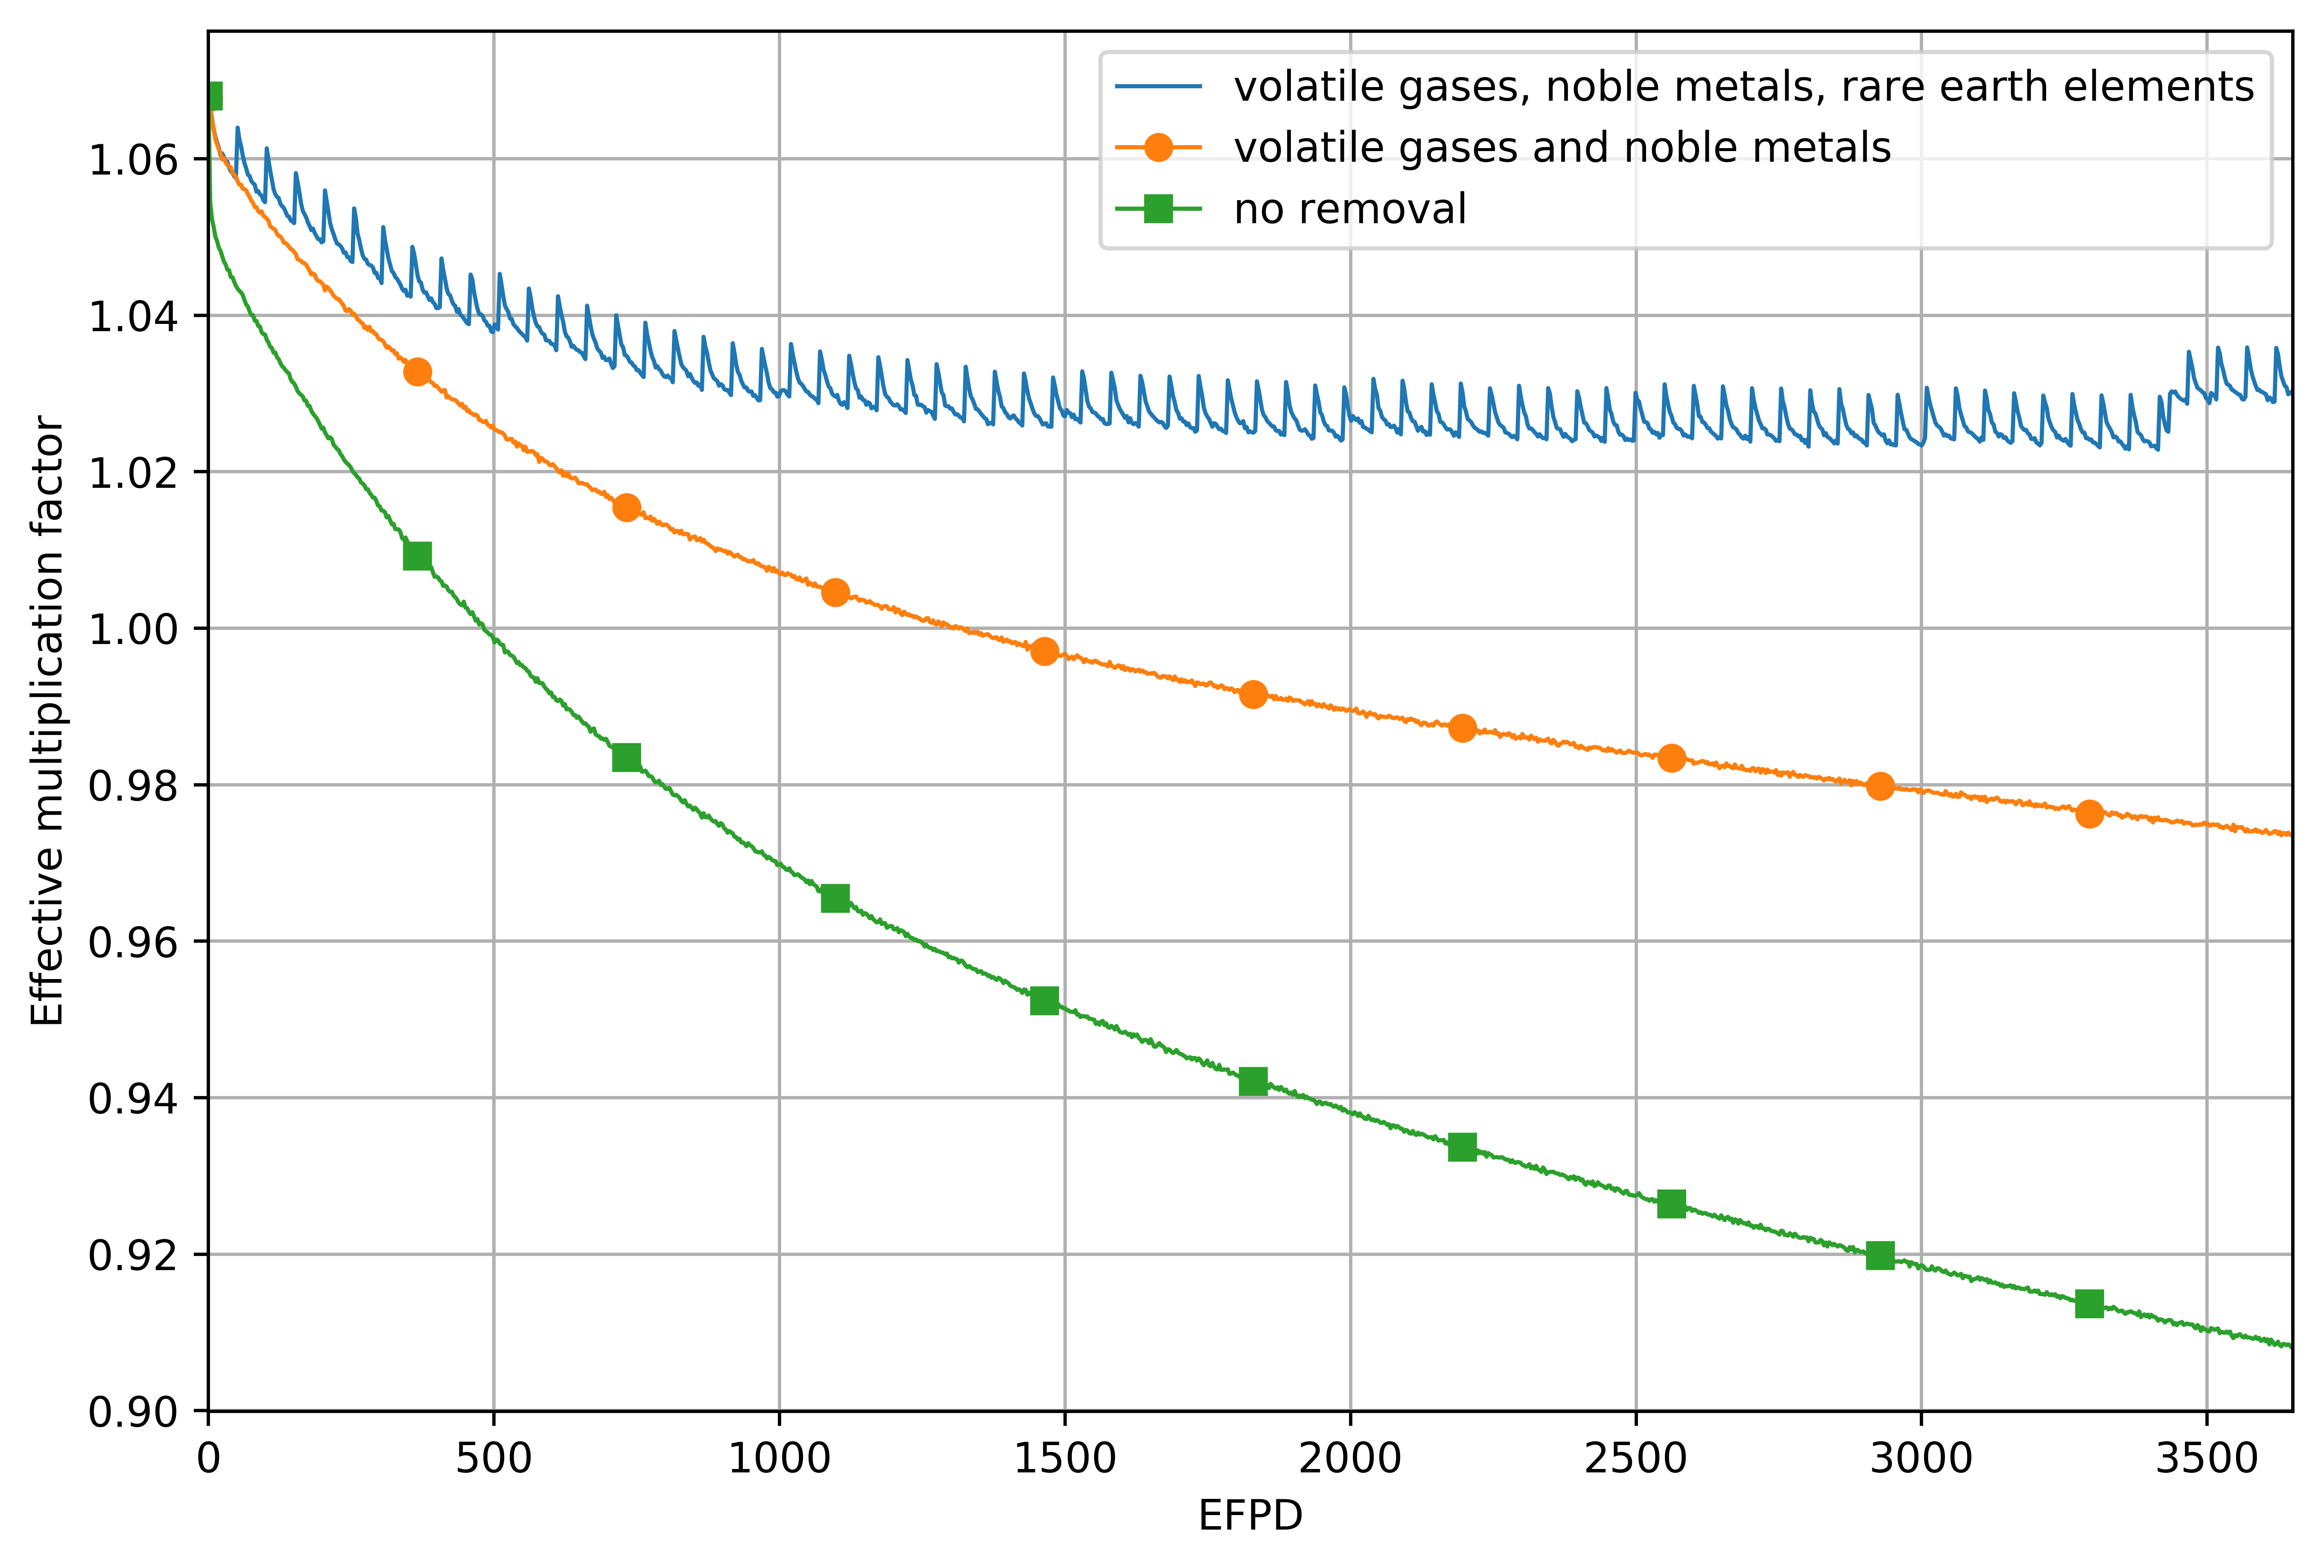
\includegraphics[width=\textwidth]{keff_rem_cases.png} 
	\caption{Calculated effective multiplication factor for full-core 
	\gls{MSBR} model with removal of various fission product groups over 10 
	years of operation (reproduced from \cite{rykhlevskii_modeling_2019}).}
	\label{fig:fp_removal}
\end{figure}

These preliminary results have demonstrated SaltProc's capability to find 
the equilibrium fuel salt composition (where equilibrium is defined as when 
the number densities of major isotopes vary by less than 1\% over several 
years). Additionally these results was showed benefits of a continuous fission 
product removal for thermal \gls{MSR} design. A full-core high-fidelity 
benchmark model of the \gls{MSBR} will be employed for demonstration and 
validation of a new version of SaltProc.
